
\documentclass[
			english,
			%review,
			]{elsarticle}
			
\bibliographystyle{elsarticle-num}
%% ======================== SETUP =========================
%% Full documentation on all packages can be found at http://google.com or with `texdoc <packagename>`


%% === Tools ==============================================
\usepackage{iftex}
\usepackage{savesym}
%%   - Silence -
%% Disable warnings that don't cause problems
\usepackage{silence}
\WarningFilter{balance}{You have called \balance in second column}
\WarningFilter{caption}{Unsupported document class}
\WarningFilter{caption}{Unused \captionsetup}
\WarningFilter{relsize}{Failed to get list}


%% === Encoding ===========================================
\ifXeTeX
  \usepackage{fontspec}
\else
  \usepackage[utf8]{inputenc}
  \usepackage[T1]{fontenc}
  \input glyphtounicode			%% Copyable unicode in pdf
  \pdfgentounicode=1
\fi


%%% === ACM Template =======================================
%%% Depending on font, may look better with `relayout`
%\usepackage[relayout]{myacm}
%\usepackage{balance}
%%%   - Default font, choose one -
%\usepackage{txfonts}			%% Times Roman, as requested by style guide, creates smaller documents
%%\usepackage[lighttt]{lmodern}	%% Latin Modern, with light typewriter, looks almost like default setting


%% === article Template ===================================
%%   - Font -
\usepackage[lighttt]{lmodern}	%% Latin Modern with light typewriter


%% === Fonts ==============================================
%%   - Other -
%\savesymbol{iint}					%% Better math font
%\savesymbol{iiint}				%
%\savesymbol{iiiint}				%
%\savesymbol{idotsint}			%
\usepackage{MnSymbol}			%% /Better math font
\usepackage[babel=true]{microtype} %% Better kerning


%% === Language ===========================================
\usepackage{babel} 							%% Select language in \documentclass
\usepackage[babel]{csquotes}		%% \enquote, \blockquote
%%   - Quotes -
%% Options for english: british -> '', american -> ""
\ExecuteQuoteOptions{french=guillemets,german=quotes,english=american}
\newcommand\q[1]{\enquote{#1}}	%% Quote with \q{}
\MakeAutoQuote{>}{<} %% {«}{»}
\MakeOuterQuote{"}


%% === Page Format ========================================
%\usepackage{fancyhdr}			%% more header and footer configuration
%\usepackage{pdflscape}			%% \begin{landscape} ... \end{landscape}


%% === Bibliography =======================================
%% use biblatex if you know what you're doing
%\usepackage[
		%%backend=bibtex, 			%% bibtex, no utf-8 support
		%backend=biber,				%% biber backend
		%style=numeric-comp,		%% [1]
		%%style=alphabetic, 		%% [Auth99]
		%%citestyle=authortitle-tcomp,
		%%bibstyle=verbose,
		%%backref=true,
		%defernumbers=true,
		%doi=false,isbn=false,url=false,
		%]{biblatex}
		
		
%% === Images =============================================
\usepackage{graphicx}			%% \includegraphics
\usepackage{subfig}				%% Sub-figures
\DeclareGraphicsExtensions{.pdf,.png,.jpg,.ai}
\DeclareGraphicsRule{.ai}{pdf}{*}{}


%% === Colors =============================================
\usepackage{color}
%\usepackage{colortbl}					%% Colors for tables
\usepackage[svgnames,table]{xcolor}		%% more colors and \rowcolors


%% === Tables =============================================
%\usepackage{ctable}				%% \ctable command
%%  - Table Style -
%% colored rows, requires xcolor
%\newcommand{\insidetable}{\rowcolors*{2}{WhiteSmoke}{white}}
%\setupctable{doinside=\insidetable}


%% === Code Listings ======================================
\usepackage{listings}
%%   - Basic Looks -
\lstset{
	captionpos=b, 
	xleftmargin=0.35cm,
	basicstyle=\smaller\ttfamily, 
	showstringspaces=false, 
	columns=fixed, 
	basewidth={0.5em,0.45em}, 
	upquote=true,
	tabsize=2, 
	gobble=2,
	escapeinside={/*@}{@*/},
	numberbychapter=false,
}
%%   - Linebreaks -
\lstset{
	breaklines=true, 
	breakatwhitespace=true,
	%prebreak=\raisebox{0ex}[0ex][0ex]{\emptyaccsupp{\small\ensuremath{\rhookswarrow}}},
	postbreak=\raisebox{0ex}[0ex][0ex]{\emptyaccsupp{\small\ensuremath{\rcurvearrowse\space}}},
}
%%   - Line Numbers -
\lstset{
	numbers=left, 
	numberstyle=\tiny\emptyaccsupp, 
	numbersep=5pt,
	numberfirstline=true, 
	firstnumber=auto, 
	stepnumber=5,
}
%%   - Copy&Paste -
\lstset{keepspaces=true}
\ifXeTeX
\else
  \makeatletter
  \def\lst@outputspace{{\ifx\lst@bkgcolor\empty\color{white}\else\lst@bkgcolor\fi\lst@visiblespace}}
  \makeatother
	\pdfglyphtounicode{visiblespace}{A0}
	\pdfglyphtounicode{blank}{A0}
	\pdfglyphtounicode{visualspace}{A0}
	\pdfglyphtounicode{uni2423}{A0}
\fi
%%   - Languages -
\lstdefinelanguage{JavaScript}{
	keywords={break, case, catch, continue, debugger, default, delete, do, else, finally, for, function, if, in, instanceof, new, return, switch, this, throw, try, typeof, var, void, while, with},
	morecomment=[l]{//},
	morecomment=[s]{/*}{*/},
	morestring=[b]',
	morestring=[b]",
	sensitive=true,
}
\lstdefinelanguage{HanaSQL}[]{SQL}{
	morekeywords={replace,string,if,daysbetween,secondsbetween,weekday,adddays,addseconds,double},
}
\lstdefinelanguage{algorithm}{
	keywords={break, case, catch, continue, dec, default, delete, do, each, else, end, error, exists, finally, for, function, if, inc, is, new, return, switch, then, this, throw, try, typeof, until, var, void, while, with},
	morestring=[b]",
	morecomment=[l]{//},
	morecomment=[s]{/*}{*/},
	moredelim=[is][\slshape]{'}{'},
	moredelim=[is][\bfseries]{''}{''},
	style=algorithmStyle,
}
\lstdefinestyle{algorithmStyle}{
  literate= % replace with math symbols
			{:=}{{\(\gets\)}}2 {~}{{\(\:\!\!\neg\)}}1
			{<=}{{\(\leq\)}}1 {>=}{{\(\geq\)}}1 
			{!=}{{\(\neq\)}}1 {=}{{\(=\)}}1
			{&&}{{\(\wedge\)}}1 {||}{{\(\vee\)}}1 
			{\{\}}{{\(\emptyset\)}}1
			{\\in}{{\(\in\)}}1
			{\\notin}{{\(\notin\)}}1
			{\\exists}{{\(\exists\)}}1
			{\\nsubseteq}{{\(\subseteq\)}}1
			{<<}{{\(\ll\)}}2
			% escape with \
			{\\:=}{{:=}}2 {\\~}{{\textasciitilde}}1
			{\\<=}{{<=}}2 {\\>=}{{>=}}2 
			{\\!=}{{!=}}2  {\\=}{{=}}1
			{\\&&}{{\&\&}}2 {\\||}{{||}}2 
			{\\\{\}}{{\{\}}}2
			{\\bs}{{\textbackslash}}1 
			{\\'}{{'}}1 
}
%%   - Styles -
\lstdefinestyle{EclipseStyle}{
	keywordstyle=\bfseries\color{Purple},
	stringstyle=\color{Blue},
	commentstyle=\color{Grey},
}
\lstdefinestyle{BWStyle}{
	keywordstyle=\bfseries,
	stringstyle=\color{DimGray},
	commentstyle=\slshape,
}
\lstset{style=BWStyle,language=Java}
\lstMakeShortInline[basicstyle=\ttfamily,language={}]´


%% === More Tools =========================================
%% no changes here
\usepackage{xspace} 			%% \xspace, automatic spaces for custom macros
\usepackage{float}				%% custom floats
\usepackage{mparhack}			%% marginpar hack
% \usepackage{fixltx2e}			%% latex bugs
\usepackage{relsize}			%% \smaller
\usepackage[space=true]{accsupp}
\newcommand\emptyaccsupp[1]{\BeginAccSupp{ActualText={}}#1\EndAccSupp{}}


%% === Misc ===============================================
\usepackage[printonlyused]{acronym}	%% Acronyms
\renewcommand*{\acsfont}[1]{\textsc{#1}}
%% pdfcomments, load before hyperref
\usepackage{pdfcomment}
%% Exclude footnote links from copy&paste
\renewcommand{\thefootnote}{\protect\BeginAccSupp{ActualText={}}\arabic{footnote}\protect\EndAccSupp{}}


%% === Links and Captions =================================
%\usepackage{hyperref}
%\hypersetup{
%%	draft,						%% disable all
	%%% better set this as document option
	%%colorlinks, 				%% color links, instead of bordered
	%hidelinks,					%% for print version
%%% - link colors -
	%linkcolor=Navy,				%% internal, default red
	%citecolor=Navy,				%% citations, default green
	%urlcolor=Purple,			%% URLs, default cyan
	%filecolor=Purple,			%% files, default magenta
%%
	%plainpages=false,
%}

\usepackage[nameinlink, noabbrev]{cleveref}	%% \cref commands
\newcommand{\lineref}[2]{\hyperref[#1]{line~\ref*{#1:#2}}}
\newcommand{\linerefn}[2]{\hyperref[#1]{line~#2}}
\newcommand{\Lineref}[2]{\hyperref[#1]{Line~\ref*{#1:#2}}}
\newcommand{\Linerefn}[2]{\hyperref[#1]{Line~#2}}

%\usepackage[all]{hypcap}
%\usepackage{caption}
%\captionsetup[table]{position=t}
%\captionsetup[subtable]{position=t}


%% === Misc 2 ============================================
\usepackage[xspace]{ellipsis}	%% \dots, load after hyperref


%% === Pdf Options =======================================
\hypersetup{
	draft
	%bookmarksopen,
	%bookmarksnumbered,
%%	pdfstartview={Fit},					%% Fit page
%%	pdfstartview={FitH},				%% Fit width
	%pdfstartview={XYZ null null 1.0},	%% 100% zoom
}

%\bibliography{references}

\usepackage{lineno}
\modulolinenumbers[5]

\journal{Science of Computer Programming}

\hypersetup{
	pdftitle={Interactive Dynamic Slicing: Tracking Infection Chains with the Slice Navigator},
	pdfauthor={Arian Treffer, Matthias Uflacker, Hasso Plattner},
	pdfsubject={},
}

%% remove in final version
\usepackage[colorinlistoftodos]{todonotes}
%\renewcommand{\todo}[2][\empty]{\pdfmargincomment[color=orange,icon=Note,subject=TODO,#1]{#2}}
%\usepackage{pdfcomment}
%\newcommand{\todo}[2][]{\pdfmargincomment[color=orange,icon=Note,subject={TODO},author={#1}]{#2}}

\begin{document}

\begin{frontmatter}

\title{Interactive Dynamic Slicing: Tracking Infection Chains with the Slice Navigator}

\author{Arian Treffer, Matthias Uflacker, Hasso Plattner}
\address{Hasso Plattner Institute, Potsdam, Germany}

%\maketitle

\begin{abstract}
%Slicing is a technique to reduce the amount of code that needs to be analyzed for a given problem. 
%
%In this paper, we present the Slice Navigator, a debugging tool for Java programs that combines dynamic slicing with back-in-time debugging data to support the debugging process in multiple ways.
%Firstly, it supports the developer's short term memory by providing a summary of relevant program state and context for the current instruction.
%Secondly, it provides an alternative to breakpoints as it can be used to control the debugger to jump to related instructions, such as the last change of a variable.
%Thirdly, it allows to directly reconfigure the slicing criteria, enabling the developer to minimize the search space of active code without interrupting the debugging workflow.
%
%The paper focuses on the UI and implementation of the Slice Navigator view and how it changes the debugging workflow.
%A performance evaluation shows the feasibility of our approach for larger programs, while a user study 
 %the Slice Navigator, a debugging tool that combines two complementary approaches to debugging, back-in-time debugging and dynamic slicing, to enrich the debugging experience in multiple ways. First, it 
Of the many tools and approaches developed to help developers find bugs in code, few are used frequently in practice.
One of the reasons for this phenomenon is that developers cannot adequately integrate such tools in their debugging workflow.

We present Interactive Dynamic Slicing, a new debugging workflow combining back-in-time debugging and dynamic slicing, in which developers iteratively reconfigure slicing criteria to minimize the search space of active code without interrupting the debugging session.
The Slice Navigator, a complementary debugging tool, enables developers to use this workflow effectively by combining debugger and slicer in one view.
Using data from slice and debugger, the Slice Navigator summarizes relevant program state and context for the current instruction.
It is designed to support developers’ short-term memory, serve as an alternative to breakpoints, and allow developers to quickly adjust the slice.

This paper focuses on the user interface and implementation of the Slice Navigator and how it changes the debugging workflow. 
A performance evaluation shows the feasibility of our approach, a user study demonstrates that developers can follow infection chains up to 40\% faster with the Slice Navigator than with a regular debugger. 
This supports our view that integrating tools can reduce barriers and create synergy effects.

\end{abstract}

\begin{keyword}
dynamic slicing, back-in-time debugging
\end{keyword}

\end{frontmatter}

\linenumbers

\section{Introduction}
\label{sec:introduction}

%\todo{rewrite as debugging-tools in practice}
% Context: debugging and slicing
In many cases, software bugs don't cause the software to fail, i.e., to deviate from expected behavior, immediately.
To actually find the bug, developers have to follow the chain of erroneous states from the observed failure backwards to the bug~\cite{zeller_why_2009}.
Many approaches exist to support this process~\cite{wong_survey_2016}.

Debuggers allow inspecting the state of a running program and understanding its impact on the program's behavior, but create a mental overhead for developers who frequently need to restart the debugging session to get to earlier points in time.
Back-in-time and "omniscient" debuggers (ODBs) remove this overhead by making it possible to follow the infection chain backwards through time~\cite{lewis_debugging_2003}.
However, developers still need to manually identify the relations between states without spending too much time in irrelevant parts of the code.
This often requires a high familiarity with the code, which is not always a given.
%
%when programmer needs better understanding, turns to debugger\\
%as knowledge grows, question change\\
%linear nature of debugger, repetitive task of restarting\\
%omniscient debugging improves productivity by reducing mental overhead\\

Weiser has shown that programmers think not only in modules, but in groups of related statements called "slices"~\cite{weiser_programmers_1982}.
Slicing is a technique to produce subsets of a program relevant to a given criterion~\cite{weiser_program_1981}.
Dynamic slicing also considers the program input, which allows removing even more irrelevant instructions~\cite{korel_dynamic_1990, agrawal_dynamic_1990}.
% Significance
It has been shown that slicing can be useful to improve developer productivity~\cite{weiser_programmers_1982, agrawal_dynamic_1990}, especially for developers dealing with very complex or unfamiliar code.

% Problem: tool integration
Slicing suffers from a similar problem as debugging:
every time the developer's question changes the slice has to be recomputed, which can interrupt the developer's flow even if it only takes a few seconds.
Furthermore, every time developers need to switch between slicer and debugger, another interruption occurs.
Interruptions can easily break developer flow~\cite{altmann_04_task_interruption_resumption_lag}, this may be one of the reasons why slicing is rarely used in practice~\cite{perscheid_studying_2017}.

We present Interactive Dynamic Slicing, a new approach that combines omniscient debugging and dynamic slicing.
While developers back-in-time-debug a dynamic slice, they can, at any point, add or adjust slicing criteria.
Changes are applied immediately, without interrupting the debugging session.
A debugging tool, the Slice Navigator, provides a unique view on the program's execution by combining relevant information from both the ODB and the slicing subsystem.

The contributions of this paper are threefold:
\begin{itemize}
	\item The \emph{Slice Navigator} is a debugging tool that bundles access to the debugger and the slicer.
		It provides context for the current instruction by showing relevant parts of the slice, allows developers to iteratively refine the slicing criteria, and serves as an alternative to breakpoints and stepping.
	\item Based on previous work, we developed a dynamic slicing algorithm allowing quick and iterative refinement of the slicing criteria to adapt the slice to changing developer questions.
		Developers can formulate their question by choosing from different dependency types that will change the outcome of the slice~\cite{treffer_dynamic_2014}.
	\item The integration of dynamic analyses directly into the debugger allows developers to use a new debugging workflow we call Interactive Dynamic Slicing. Developers can isolate a bug by iteratively slicing away correct code, homing in on the problem.
	This reduces interruptions in developer flow by minimizing context switches between tools and shortens waiting time as recorded run-time data can be reused.
\end{itemize}

The remainder of this paper is structured as follows:
The next section summarizes related work.
\Cref{sec:workflow} explains the Slice Navigator user interface and how it enables developers to use Interactive Dynamic Slicing.
\Cref{sec:impl} discusses relevant details of the implementation and the slicing algorithm.
\Cref{sec:eval} evaluates the feasibility of our approach and presents the results of a user study.
\Cref{sec:conclusion} concludes.

\section{Related Work}

The concept of slicing was introduced by Weiser and initially only built on static analysis~\cite{weiser_programmers_1982, weiser_program_1981}.
Later, Korel and Laski~\cite{korel_dynamic_1990} and Agrawal and Horgan~\cite{agrawal_dynamic_1990} independently introduced dynamic slicing by proposing different ways of extending the concept to the run time~\cite{binkley_theoretical_2006}.
Quasi static slicing combines both approaches~\cite{venkatesh_semantic_1991} and simultaneous dynamic slicing~\cite{hall_automatic_1995} creates generalized dynamic slices by slicing multiple executions at once.

Many slicing algorithms have been developed for the different approaches, improving the performance~\cite{reps_speeding_1994} or precision~\cite{kumar_better_2002, zhang_precise_2003} of previous work.
An overview of algorithm types is given in~\cite{korel_dynamic_1998}.
JSlice~\cite{wang_dynamic_2008} and JavaSlicer~\cite{hammacher_08_design_and_implementation} are other dynamic slicers for Java.
The algorithm used by the Slice Navigator is based on our previous work~\cite{treffer_dynamic_2014}.
%It uses Soot~\cite{lam_11_the_soot_framework} for static analysis.

The idea of being able to debug backwards in time dates back to the 1960s with EXDAMS, a debugger for FORTRAN~\cite{balzer_exdams_1969}.
Since then, debuggers with back-in-time capabilities have been implemented for many programming languages~\cite{feldman_igor_1988, agrawal_debugging_1993, lieberman_zstep_1997, hofer_design_2006}.

In 2003, Lewis introduced the concept of "omniscient debugging", a debugger that can not only rewind time, but has instant access to every program state in the past and future~\cite{lewis_debugging_2003}.
Later work on omniscient debugging focused mostly on handling the large amounts of data such a debugger creates~\cite{pothier_scalable_2007, lienhard_practical_2008}.

Perscheid combined back-in-time debugging, incremental dynamic analysis, and spectrum-based fault localization to navigate developers semi-automatically along identified infection chains from observable failures back to their root causes~\cite{perscheid_testdriven_2013}.

SPYDER is a debugger with slicing and back-and-time capabilities~\cite{agrawal_debugging_1993}.
With SPYDER, Agrawal et al.\ also proposed a new debugging workflow that is similar to our approach.
However, while Agrawal et al.\ proposed to create a new slice every time the programmer's question changed, our approach focuses on iteratively modifying a single slice.
This way, fine-grained configuration can be retained, leading to smaller slices.
Furthermore, we present a new way of presenting aspects of the slice to developers.

Studies show that modern fault localization techniques are not widely used in practice~\cite{perscheid_studying_2017}.
Accessibility was reported as the most important feature for the adoption of debugging tools.
For us, this demonstrates a need for better integration with IDEs, other tools, and the general debugging workflow.

\section{Interactive Dynamic Slicing}
\label{sec:workflow}

Slicing can be used for many purposes, such as code optimization or automatic fault detection, e.g., to find security flaws~\cite{Ottenstein:1984:PDG:390011.808263, Backes:2016:RLA:2897845.2897927}.
In our work, we consider only the use-case of using slicing to support developers debugging a program.
In this section, we introduce configurable slicing, an extension to existing slicing approaches. 
Then we describe the user interface of the Slice Navigator, how it presents information about the slice, and how it can be used to control the debugger.
Based on configurable slicing and the Slice Navigator, we introduce a new debugging workflow called Interactive Dynamic Slicing.

\subsection{Configurable Slicing}

There a many different approaches to compute slices.
On successful method is slicing based on dependence graphs \cite{korel_dynamic_1998}.
A dependence graph-based slicing algorithm has to do three things, as illustrated in \cref{fig:graph-slicing}:
first, compute a dependence graph, then, map the slicing criteria to nodes in the graph, and finally, collect the transitive dependencies of the initial nodes.

\begin{figure}
	\centering
		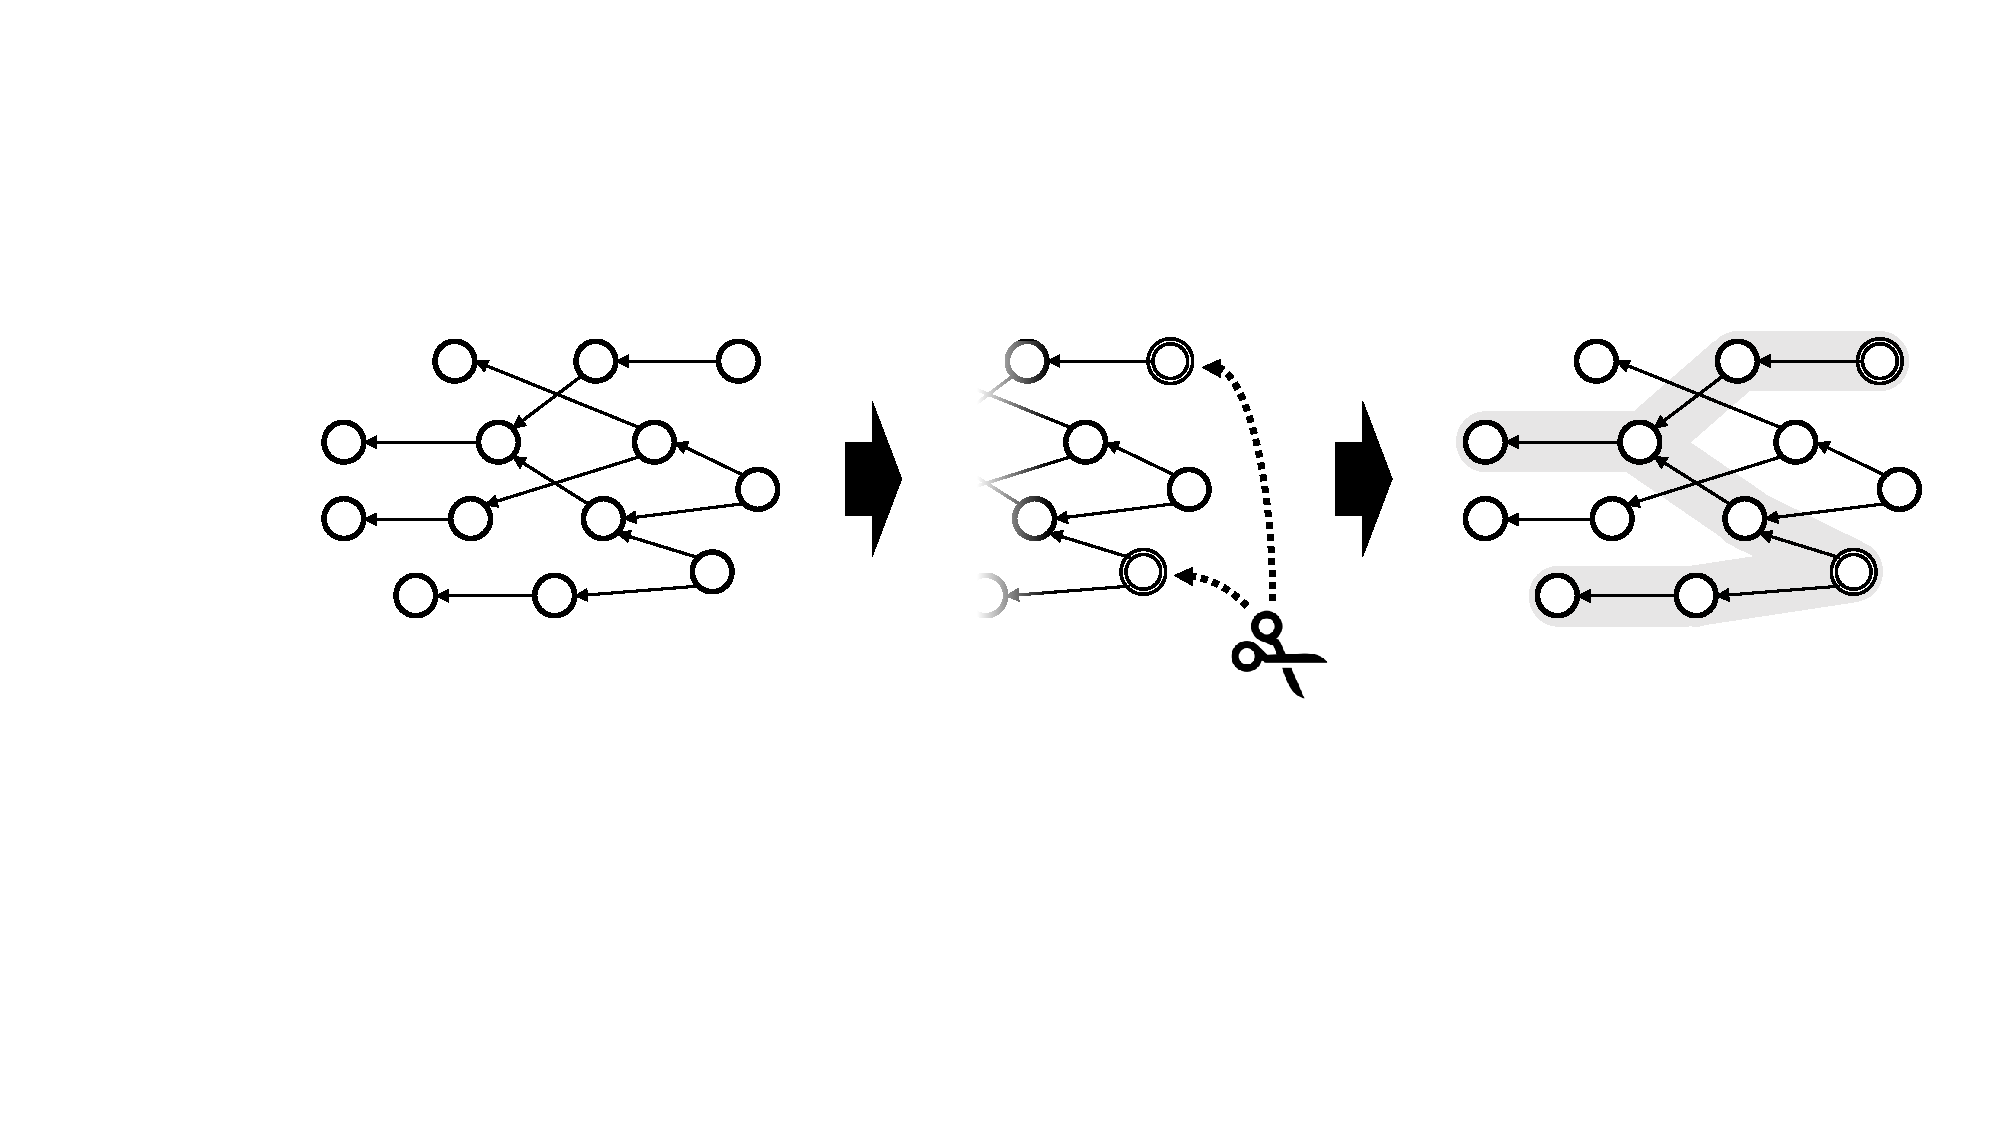
\includegraphics[width=\linewidth]{graph-slicing}
	\caption{Deriving a slice from a dependence graph in three steps: compute the graph, map the criteria, and collect the dependencies.}
	\label{fig:graph-slicing}
\end{figure}

Slicing algorithms do not necessarily perform these steps in a distinct order, but may already map nodes and collect dependencies while the graph is constructed~\cite{agrawal_dynamic_1990,zhang_precise_2003}.
Nevertheless, each step of the algorithm fits one of these three purposes.

Depending on the algorithm, different types of graphs can be used.
For example, a static slicing algorithm would use a program or system dependence graph, where each node represents an instruction, whereas a dynamic slicing algorithm would use a dynamic dependence graph, where each node represents the execution of an instruction~\cite{weiser_program_1981, korel_dynamic_1990}.
Regardless of their type, dependence graphs can contain different types of dependency relations.
Two dependency types commonly used are data dependencies to model the data flow of an application and control dependencies to model its control flow \cite{weiser_program_1981, agrawal_dynamic_1990, zhang_precise_2003, korel_dynamic_1990}.

Slicing algorithms have to balance between two conflicting requirements: 
on the one hand, the slice should be as small as possible to reduce the search space for developers,
on the other hand, it is crucial that the instruction the developers is looking for is not removed.
It has been recognized that safely producing smaller slices requires additional knowledge about the developer's question beyond the pure slicing criteria.
For some classes of questions, e.g, "how was this value computed", it can be helpful to construct a dependence graph with dependencies of only one type, such as data dependencies.
Tools that can provide such reduced slices can improve debugging efficiency as less code has to be inspected by developers~\cite{agrawal_debugging_1993, Sridharan:2007:TS:1273442.1250748}.

%Regarding slicing criteria, some algorithms are limited to criteria that can be directly mapped to nodes in the graph, such as value assignments, while other algorithms can map a wider range of criteria, such a variable value in a line where it is not used~\cite{korel_dynamic_1990, agrawal_dynamic_1990}.

We propose to generalize this approach by moving the dependency type selection from the first step (dependence graph creation) to the third step (transitive dependency collection).
We call this new way to collect dependencies "configurable slicing".
Since it affects only the last step, it can be considered as an extension to all graph-based slicing approaches, regardless of the graph type and how criteria are mapped.

\paragraph{Definitions} Let $N$ be the set of nodes in a dependence graph, $T$ the set of dependency types, $D \in N \times N \times T$ the set of typed dependency edges, and $DG = (N, D)$ the typed dependence graph. A slicing criterion is commonly defined as $c = (n, V, ...)$, where $n \in N$ is a node in the graph, $V$ is a set of variables whose values must be preserved at $n$, and "$...$" represents additional arguments that a specific approach might require.
The concrete values of $N$ and $D$ can depend on the chosen criteria.
Their values are defined by the underlying slicing approach and not further discussed here.

Extending the existing definition, we define a configured slicing criterion \linebreak $c' = (n, V, ..., T_n)$, where $T_n \subseteq T$ is a subset of dependency types chosen for a specific node.
The configured dependency set of a node is 
\[dep_C(n) = \{n'\, |\, \exists\, t \in types_C(n)\mbox{: } (n, n', t) \in D\},
\] 
where $C$ is a set of slicing criteria and $types_C$ is a function that assigns dependency types to each node, defined as:
	\[
	types_C(n) = \begin{cases} 
	T_n& \mbox{if } (n, V, ..., T_n) \in C \mbox{ exists}
	\\
	\{t \, |\, \exists\, n' \mbox{: } n \in dep_C(n') \wedge t \in types_C(n')\} & \mbox{otherwise.}
	\end{cases}
\]
In other words, if a node is part of a slicing criterion, its dependency types are defined by that criterion, otherwise it inherits the dependency types from all nodes it is a dependency of.
Finally, we define a configured slice as
\[Slice(C) = \{n\, |\, types_C(n) \neq \varnothing\},
\]
i.e., as the set of all nodes with a non-empty set of dependency types.

\begin{figure}
	\centering
		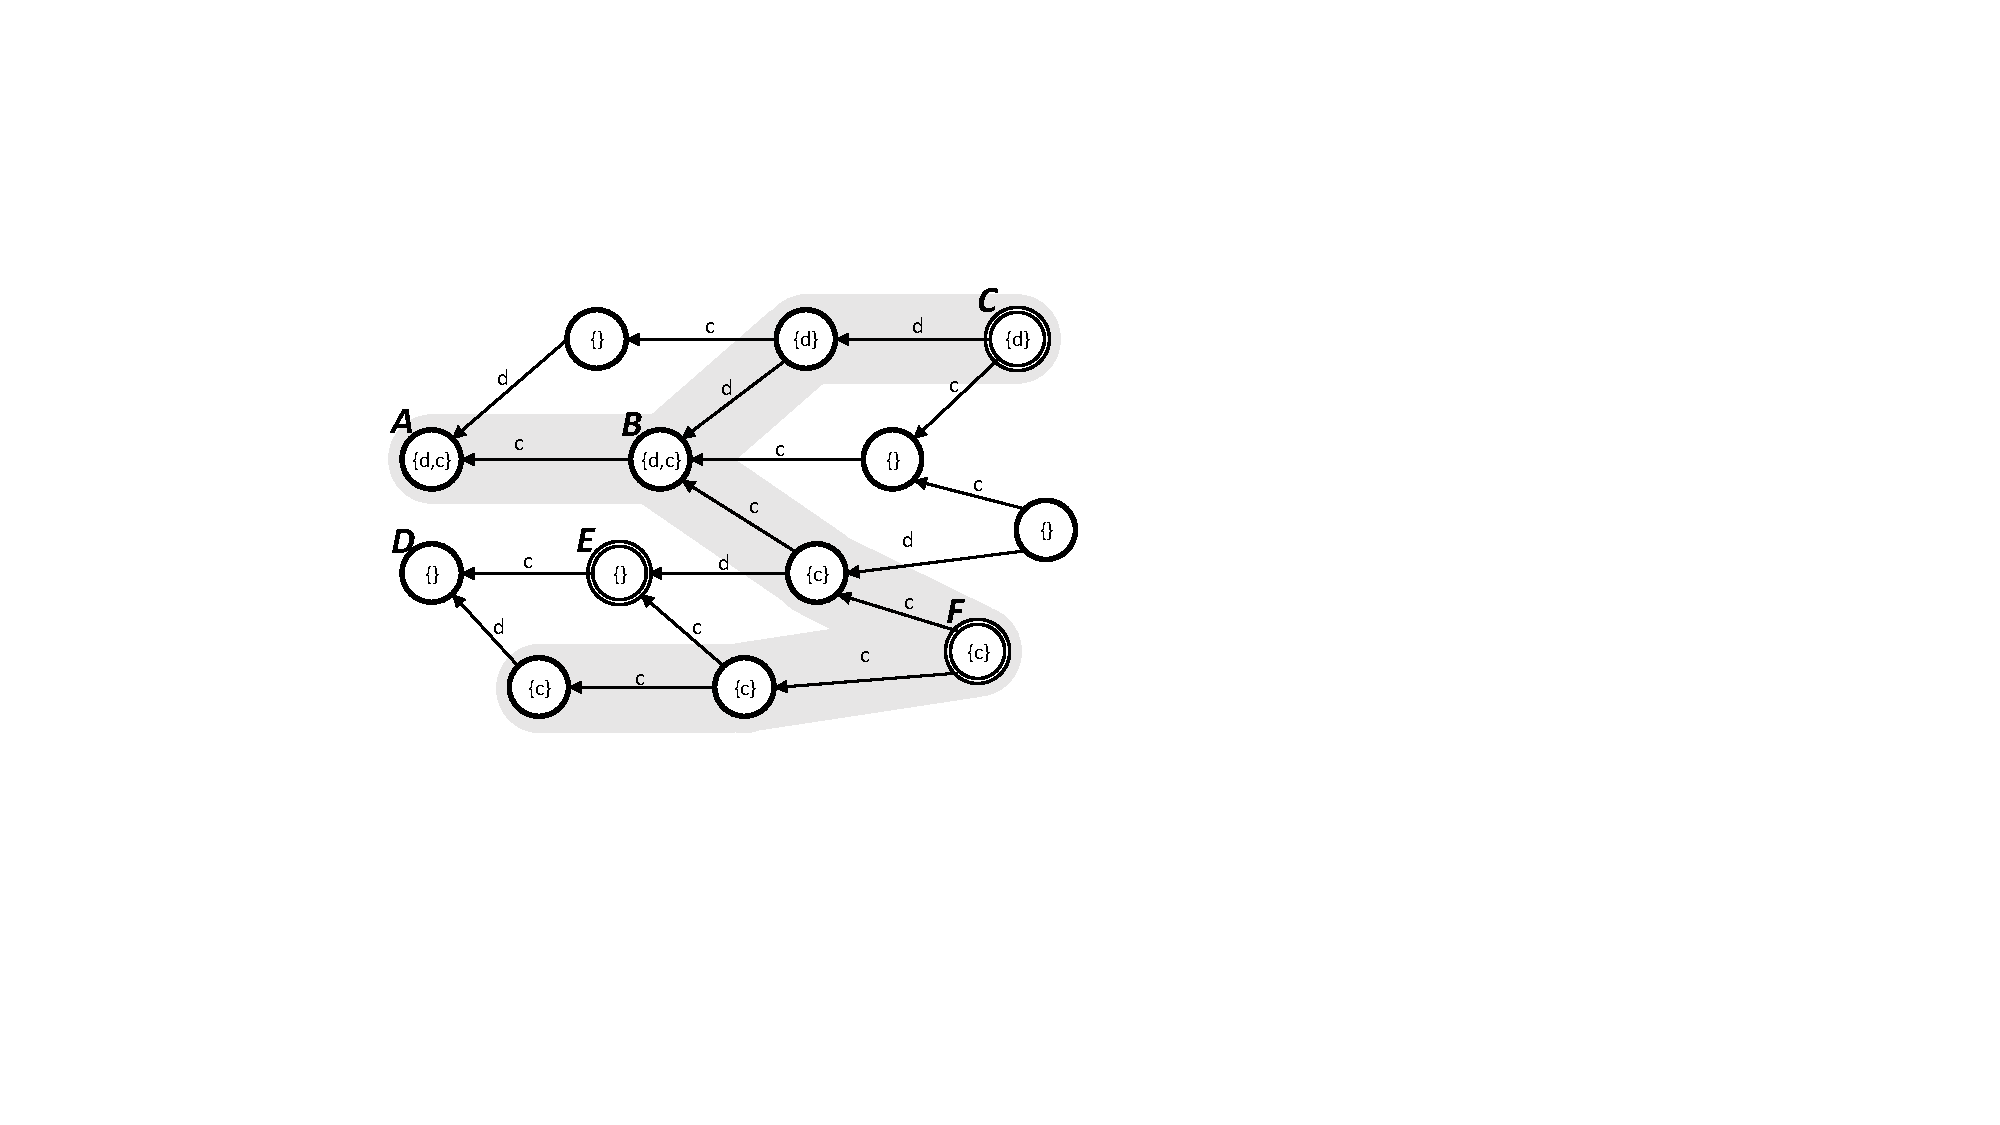
\includegraphics[width=0.60\linewidth]{configured-slice}
	\caption{A configured slice on a dependence graph with data (d) and control (c) dependencies.}
	\label{fig:configured-slice}
\end{figure}

To illustrate, \cref{fig:configured-slice} shows an example dependence graph with data and control dependencies.
Nodes \emph{C}, \emph{E}, and \emph{F} where chosen as slicing criteria.
The chosen dependency types are shown inside each node.
As can be seen, nodes \emph{C} and \emph{F} pass their respective dependency type along the according dependency edges.
Node \emph{B} inherits both dependency types and passes both to node \emph{A}, the type of the edge does not matter in this regard.
Node \emph{E} is a \emph{negative slicing criterion}.
Because its type set was chosen to be empty, not only is it excluded from the slice, it also prevents node \emph{D} from transitively inheriting the control dependency type from node \emph{F}.
The final slice is shown in gray.

It should be noted that configured slices are no longer correct with respect to the correctness definition of the underlying slicing approach.
This is acceptable as the "incorrectness" is introduced at the specific request of the developer to reduce the size of the slice.
In particular, using negative slicing criteria allows developers to exclude entire sub-graphs, for example to remove the history of values that are known to be correct.

Configurable slicing gives developers very fine-grained control over the resulting slices.
However, to utilize this control developers need to specify more detailed criteria, it is no longer sufficient to just select code locations of interest.
We do not expect developers to know beforehand which criteria configuration will yield the best slice for their purposes.
Instead, with Interactive Dynamic Slicing, we propose a method how developers can refine a slice as often as needed.

\subsection{Getting Started}

Both omniscient debugging and (dynamic) slicing changed the way how developers approach fault localization.
We use a simple example to demonstrate how we integrated both techniques into an improved debugging workflow.
%We also describe the user interface of the Slice Navigator, how it presents information about the slice, and how it can be used to control the debugger.

Very often, the starting point for a debugging session is a reproducible observable program failure, preferably in the form of a failing unit test.
Using an omniscient debugger, developers halt the execution at the failing line of code to observe the program state.
From here, they want to backtrack the erroneous state.
However, they quickly realize that the code contains many other side effects making it hard to follow the state of interest.

Using a pure omniscient debugger, developers would now have to track the relation of states to identify the infection chain. 
In other words, they have to manually create a dynamic dependence graph, i.e., the dependencies between statement executions~\cite{korel_dynamic_1990}, using only their short-term memory. 
When slicing features are supported, they might rather leave that task to the tools.
In our user study, where we tested our approach on real open source programs, the initial slice already removed between 70 and 85\% of the code.
In large and complex applications, however, such a slice might still be too large to be practical~\cite{agrawal_dynamic_1990, Sridharan:2007:TS:1273442.1250748}.

%\interfootnotelinepenalty=10000
%We will use a small code example to explain the user interface and internals of the Slice Navigator. 
To illustrate this problem, we will use a small example where the resulting slice contains almost the entire program.
\Cref{lst:example}
%\footnote{In "review" mode, the Elsevier LaTeX template places listings at the end of the document. This will be changed in the final layout.} 
shows two Java classes and a JUnit test case. %TODO reword minimal example
A bug in line 17 prevents the initialization of a field and the unit test fails accordingly.
In our scenario, after noticing a failed test case, developers choose to slice on the arguments of the ´assertEquals´ invocation in \linerefn{lst:example}{31}.



\begin{lstlisting}[float,label=lst:example,caption={Example program with a failing test case}]
	class Square implements Shape2D {
		private double length;
		public Square(double length) { 
		  this.length = length;
		}
		
		@Override
		public double getArea() { 
			return length * length;
		}
	}
	
	class Pyramid implements Shape3D {
		private Shape2D base;
		private double height;
		public Pyramid(Shape2D baseShape, double height) {
			base = baseShape;
			height = height;
		}
		
		@Override
		public double getVolume() { 
			return base.getArea() * height / 3; 
		}
	}
	
	class PyramidTest {
		@Test
		public void test_getVolume() {
			Shape3D shape = new Pyramid(new Square(2), 6);
			assertEquals(8, shape.getVolume());
		}
	}
\end{lstlisting}


Using our tool, a plug-in for the Eclipse IDE, developers can right-click the erroneous state in the debugger's variables view and choose slicing from the context menu.
This will set the variable or field as a slicing criterion and start the slice computation.
%The initial code analysis can take a few seconds.
%The performance of our prototype implementation is evaluated in \todo{section ?} .
Once the slice is computed, all debugging views (e.g., the trace and the variable view) will gray out instructions or variables not belonging to the slice.
Stepping through the execution will skip excluded instructions accordingly.
Last but not least, the IDE opens the Slice Navigator, a UI component that assists developers debugging the slice.


%However, the size of the initial slice is not very important. 
%For a complex program, it is likely too large to allow an efficient search for the problem.
%In this case, the developer can now use the Slice Navigator to get an overview of the execution and to iteratively adjust the slicing criteria.

\subsection{The Slice Navigator}
\label{sec:the_slice_navigator}

To produce a slice, dynamic or static, slicing tools have to build up deep knowledge of a program's internal workings.
In the end, only a binary mapping about which instruction to include or exclude from the program is returned, and most of the slicer's internal knowledge is discarded.
Hence, the initial motivation for the Slice Navigator was to make better use of a slicer's internal data.
However, since the size of the entire dynamic dependency graph is typically too vast to be visualized at once, we propose to use this data to guide developers while they debug the slice.

The first purpose of the Slice Navigator is to aid the developer's short-term memory.
It provides a quick overview of previous and upcoming events, and how they relate to the current instruction.
\Cref{fig:slice1} shows a screenshot of the slice navigator with the execution of the example test-case halted on the ´return´ instruction of ´getArea()´ in \linerefn{lst:example}{7}.

\begin{figure}
  % picture on first page :)
	\centering
		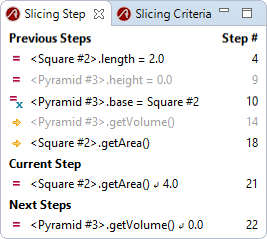
\includegraphics[width=0.40\linewidth]{slice1.png}
	\caption{The Slice Navigator shows context for the current debug step. Steps directly related to the current step are listed in black, steps with overarching dependencies in gray. Small icons indicate how the steps are related.}
	\label{fig:slice1}
\end{figure}

A step, or event, is the execution of any instruction or statement that has a side effect on the program state, or a method invocation or return.
"Previous Steps" lists all past events that the current or any future events depend on.
Likewise, "Next Steps" shows all events that depend on the current or a previous event.

If a step is shown in black, it has a direct dependency link to the current step.
Steps shown in gray have dependencies that go beyond the current step, i.e., gray "previous steps" have dependency links to "next steps", and vice versa.

Simply by looking at the previous and next steps, the developer can understand at a glace how the current instruction fits into the greater scheme.
This is particularly useful if the current instruction was reached via a breakpoint, in which case it is not always obvious at which point in time it was hit.

To obtain this kind of information with a regular debugger, developers need to analyze the execution stack and maybe even inspect lower stack frames.
But even then it is not always obvious which part of the reachable program state is actually used again.
Unlike a typical debugger's variable view, the Slice Navigator only shows relevant variables, and also shows relevant object fields on the first level.

Furthermore, the Slice Navigator shows small icons indicating how the events are related.
%The icons reveal details about the dependency graph that was used to compute the current slice and will be explained in the next subsection.
In our prototype, we distinguish between three types of dependencies: data and control dependencies, as described above and used by many authors~\cite{weiser_program_1981, agrawal_dynamic_1990, zhang_precise_2003, korel_dynamic_1990}, and a new dependency type called "choice dependency".

\emph{Data dependencies}, shown as a red equality sign, represent regular dataflow.
In variable and field assignments, the left side has a value dependency to the expression on the right, method arguments depend on the respective expression on the call site, and method results depend on the return expression.

Instructions that determine if or how another instruction can be reached are \emph{control dependencies}, indicated by a yellow arrow.
Every event except the root invocation has at least one control dependency.
For method invocation events it is the method call on the call site, for all other events it is either the enclosing method invocation or the conditional expression of an \emph{if} or loop statement.

Sometimes, a value depends on only one of multiple candidate data dependencies. 
A \emph{choice dependency} determines which of these candidates is used.
More formally, choice dependencies are all control dependencies of data dependency candidates that are not also control dependencies of all other candidates.
In the navigator, choice dependencies are indicated by a blue~"X".
It should be noted that slicing algorithms typically do not track this type of dependency as it is redundant for the purpose of slice computation.
However, we believe there is an additional value for developers in showing these dependencies.
As we discussed before, data and control dependencies can be used to answer different questions about the code.
The choice dependency captures a pattern where a control dependency acts more like a data dependency.
Explicitly tracking choice dependencies gives developers more control over the resulting slice. %For instance, to determine how a value was computed, they can request a slice without control dependencies except

% TODO: choice are between data and control, 

\subsection{A New Debugging Workflow}

The second purpose of the Slice Navigator is to serve as a convenient interface to the debugger.
%Debugging with the Slice Navigator is simple:
To investigate the origin of a value, developers can simply click it to move the execution to that point in time.
This way, the Slice Navigator allows developers to efficiently follow infection chains of erroneous states.
Likewise, it is easy to follow up on the impact of an instruction by navigating to its future dependencies.

As developers continue to debug, their understanding of the program and their questions change.
The initial slice will at some point no longer fit those questions.

Thus, the Slice Navigator's third purpose is to allow developers to quickly adjust the slicing criteria.
Configurable slicing uses different dependency types to adjust the slice for specific purposes, but requires developers to chose these types for each criterion.
So far, it all dependency types were selected by default.
In the Slice Navigator, developers can click an event's dependency symbol to brings up a dialog that allows to choose which dependencies of that event to include.

%Clicking on an event's dependency symbol brings up a dialog that allows to choose which dependencies of that event to include.
%This way developers can, for instance, put a focus on how a value was computed or why an instruction was reached.
%It is also possible to remove all dependencies of an event, for instance if it is known to be correct and its history is not of interest, thereby moving the focus of the slice to less well-understood parts of the program.

\begin{figure}
	\centering
		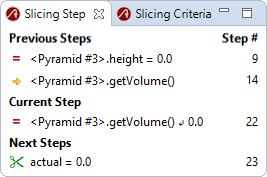
\includegraphics[width=0.40\linewidth]{slice2.png}
	\caption{The program halted at \linerefn{lst:example}{21}, after \lstinline{getArea()} was removed from the slice.}
	\label{fig:slice2}
\end{figure}

Whenever a slicing criterion is modified, the slice is updated without locking the user interface or resetting the current debugging session.
In our examples, developers might choose to exclude the result of ´getArea()´ from the slice because it is correct.
As shown in \cref{fig:slice2}, with the computation of the area removed from the slice it is now much easier to see that the wrong result of ´getVolume()´ was caused by a wrong value in the ´height´ field.

As mentioned before, instructions and states not belonging to the slice are still shown in the IDE, mostly to serve as an orientation help, to provide context to the current operations.
However, it might also happen that a value or instruction outside of the slice catches a developers attention.
In this case, they can choose to add it as another slicing criterion and the slice is expanded.
Again, this happens without interrupting the developer's work.

After some preliminary user testing, we added two shortcuts for frequently used operations.
Right-clicking an entry sets it as a negative slicing criterion, allowing developers to quickly trim the slice. 
Double-clicking an entry sets it as a slicing criterion and removes all previous non-negative criteria.
This basically starts a new slice but remembers which parts of the program developers already specified as not relevant.

With the power to quickly modify the slice as needed and with currently relevant dependencies laid out, developers can efficiently reduce the search space for a fault.
This sums up the debugging workflow we call Interactive Dynamic Slicing.
With the necessary tools integrated in the IDE, it is designed to be easily adopted by developers who follow the scientific approach to debugging~\cite{araki91:a_general_framework}.

For instance, let us assume a group of developers who are reluctant to use omniscient debugging because of the overhead it imposes~\cite{lewis_debugging_2003, pothier_scalable_2007, perscheid_studying_2017}.
They will only use it when a bug is particularly hard to locate or an infection chain is difficult to follow, so that not having to frequently restart the debugger outweighs the overhead of the ODB.
With slicing directly integrated in the debugger, there is no additional barrier to give it a try.
Because our tool never freezes the UI or otherwise interrupts developers, in the worst case scenario the slice is just not very useful, but this alone is not a big deterrent to trying it again.

While debugging the slice, developers might occasionally find the information provided by the Slice Navigator useful, more so as they become more familiar with the UI.
With the Slice Navigator more in the focus, developers can discover how it can be used to control the debugger and slice.
Over time, the developers become more effective at using slicing.
Following the scientific debugging method, every time the developers have to adjust their working hypothesis, they can adjust the slice accordingly.
This increases the usefulness of the ODB as well and hopefully leads to developers using both techniques more often.

\section{Prototype Implementation}
\label{sec:impl}

The Slice Navigator is part of a set of debugging tools that we implemented as a plug-in for the Eclipse IDE.

\subsection{Framework}

The high-level architecture of our prototype consists of three components: the tracer, the event database, and the omniscient debugger including the slicing module.

The tracer is implemented as a Java agent that modifies the bytecode of a program to insert tracing instructions that log all events.
With our Eclipse plug-in, the developer can initiate an omniscient debugging session by selecting a customized launcher in the run configuration.
The launcher will add VM arguments to the execution to configure the tracer.
Once the execution completes, the launcher will automatically import the trace data into a previously configured database.
We provide launchers for basic Java applications and for JUnit test suites.
For JUnit launches, the tracer will treat each test case as an independent execution and ignore code of the testing framework.

The database stores all events of a set of executions.
It is possible to set up one database per project or one for the entire workspace.
We currently support HSQLDB, MySQL, and SAP Hana, but in principle any relational database can be used.

The omniscient debugger consists of a set of Eclipse views that allow to debug a Java application based on the data from the database.
It is a post-mortem debugger, i.e., it simulates a debugging session while the actual program has already terminated.

\subsection{Initial Slice Computation}

In principle, the Slice Navigator can run on top of any slicing algorithm that supports configurable slicing.
However, to maximize its effectiveness, the algorithm should satisfy three criteria:
First, it should be able to quickly produce useful results to avoid interrupting developers in their work.
Waiting too long for results can easily impair developer productivity and a quickly computed incomplete slice might be more useful than a complete slice after many seconds of waiting.
%Second, it should distinguish between different types of dependencies that are easy to understand and useful for developers.
Second, it should distinguish between different types of dependencies that provide benefits to developers.
Configurable slicing is only helpful when dependency types match the developers' model of the program, the same applies to information shown in the Slice Navigator.
%additional helpful information can be communicated to the user and better customization of the slice is possible.
Finally, the algorithm should support incrementally changing the slicing criteria.
While it may be acceptable to wait several seconds for the initial slice, slow incremental changes will discourage developers from using configurable slicing to the fullest extent.

The algorithm we use in our prototype is based on previous work~\cite{treffer_dynamic_2014} and was specifically engineered to meet these criteria.
It combines method-level program dependence graphs with an execution trace to build a dynamic dependence graph.
The basic structure of the algorithm for building the initial slice is summarized in \cref{lst:slicealgo}.

\begin{lstlisting}[float=t,language=algorithm,label=lst:slicealgo,caption={Simplified algorithm for building the slice}]
	function build_slice(criteria)
		slice := {}
		for each event \in criteria do
			''asynchronous:'' add_to_slice(slice, event)
		return slice
		
	function add_to_slice(slice, event)
	  if event \in slice || event.is_negative_criterion then return
		slice += {event}
		static_dependency_graph := event.method.dependency_graph
		static_dependencies := static_dependency_graph.get(event.instruction, event.dependency_flags)
		for each dependency_link \in static_dependencies do
			for each prev_event \in previous_events(event, dependency_link) do
			  prev_event.inherit_dependency_flags(event)
				''asynchronous:'' add_to_slice(slice, prev_event)
\end{lstlisting}

%\begin{lstlisting}[numberfirstline=true,language=algorithm,firstnumber=1,label=lst:slicealgo,caption={Example program with a failing test case}]
	%function build_slice(criteria)
		%slice := {}
		%for each event \in criteria do ''in parallel''
			%add_to_slice(slice, event)
		%return slice
		%
	%function add_to_slice(slice, event)
		%'add event to slice'
		%'get static dependency graph of event\'s method'
		%'get static dependencies of event\'s instruction'
		%for each instruction \in 'static dependencies' do ''in parallel''
			%'find last previous event at instruction'
			%if 'previous event exists' && 'previous event' \notin slice then
				%add_to_slice(slice, 'previous event')
%\end{lstlisting}

%A static code analysis built with the Soot framework creates static dependency graphs on the method level.
%Static dependency graphs are computed on demand and cached for reuse.

The slicing criteria are a set of events, the slice is initially an empty set.
For each event that is added to the slice, the static dependency graph of the event's method is obtained.

If the static dependency graph is not initialized yet, it will be created by a code analysis using the Soot framework\footnote{\url{https://sable.github.io/soot/}}~\cite{lam_11_the_soot_framework}.
The graph contains every instruction's static dependencies and distinguishes between data, control, and choice dependencies.
%To handle reflection, special cases are implemented at two points.
%First, the tracing agent does not trace the internals of reflection methods such as Field\#set or Method\#invoke, but generates a simple corresponding event instead.
%Second, the static dependency graph for those methods is hard-coded to correctly link the even with the method arguments.
In the graph, dependency links are looked up by the event's instruction. 
If a value was potentially assigned in multiple locations, i.e. when branching is involved, the dependency link contains a structure describing all possibilities.
In other cases it contains only one entry.
For each dependency link, the latest matching events are looked up in the event database.
This look-up ensures that only events where a dependence exists at run time are included, leading to precise slices~\cite{zhang_precise_2003}.

For variable assignments the look-up is limited to the current method invocation, for events like field assignments the scope is not limited.
If an event is found, it is added to the slice next.

Every event carries flags that indicate which types of its dependencies the slice should include.
If the dependency flags are empty, the event is considered a negative criterion and removed from the slice entirely (cf.~\linerefn{lst:slicealgo}{8}).
If the dependency flags of an event were not configured directly by the user, they are inherited from the depending events (cf.~\linerefn{lst:slicealgo}{15}).

As can be seen, the algorithm is designed to follow all dependency links concurrently.
This allows using parallelization to improve the performance of the slicer.
The amount of concurrency is only limited by the theoretical maximum level of concurrency in the original program.
This is to be expected as the slicer is, in some sense, just evaluating the program backwards.

We also let the slicing run concurrently to the user interface.
Twice per second, we update the different debugging views, such as variable and trace explorer, to use the latest intermediate result.
This way, we not only avoid freezing the user interface, but we can allow developers to begin working with an incomplete slice immediately, even if computing the whole slice takes longer than developers are willing to wait.

\subsection{Incremental Slicing}

Adding another event to the slicing criteria works similarly to building a new slice, the major difference being that the slice is not initially empty.

When developers want to remove an event from the slice, we need to know when to cascade the removal to its dependencies.
As the dependency graph is acyclic, we can use reference counting for this.
However, we need to independently count the references for each dependency type.
When the counter for one of the dependency types reaches zero, dependencies of that type are unlinked respectively.

Changing the dependency type of an event, e.g., from data to control, is a combination of removing and adding an event, respectively.

\subsection{Filling the Slice Navigator}

To fill the Slice Navigator, we iterate over the events in the slice, ordered by step number, beginning at the current step, and collect the events to be shown.
Events directly related to the current step will be flagged as such, so that they can be highlighted.

Events at the current step and their dependencies are always collected.
For events in the future, it is first determined whether they have direct dependencies that are in the past.
If such dependencies exist, they are collected together with their respective future event.

However, our collection algorithm considers two special cases:

First, control dependencies are collected only for the current step.
This measure is taken to prevent the entire method stack from appearing in "previous steps" and all future variable changes in "next steps".

The second special case are transparent classes.
Classes of the JDK are flagged as transparent.
All their internal events, i.e., all events except direct accesses from non-transparent classes, are resolved immediately and never appear in the navigator.
This keeps the focus on the actual program and alleviates developers from having to debug through library code.

\section{Evaluation}
\label{sec:eval}

We evaluated our approach in two ways.
First, we measured the run time of the slicing component for various operations on a real-world project and found it to be fast enough to be usable in practice.
Second, we let developers locate bugs using different tools and interviewed them about their experience.
The experiment confirmed the effectiveness of Interactive Dynamic Slicing and provided suggestions to further improve the usability of our approach.

\subsection{Performance Considerations}

One of the main advantages of the Slice Navigator is that it integrates into the debugging workflow.
As such, it is crucial that results are produced in a timely manner, as a waiting time of even a few seconds may interrupt developers in their flow.

To evaluate the performance of our approach on real-world code, we measured the computation of several slices on JUnit tests of an open-source business-process engine\footnote{\url{https://github.com/camunda/camunda-bpm-platform}}.
All tests were run on a 2.0 GHz Intel i7 Processor with 4 cores and 8 GB RAM, running Windows 8.1.
A MySQL database was used to store the trace data.
We repeated every measurement 10 times, all charts show the mean values.

\begin{figure}
	\centering
		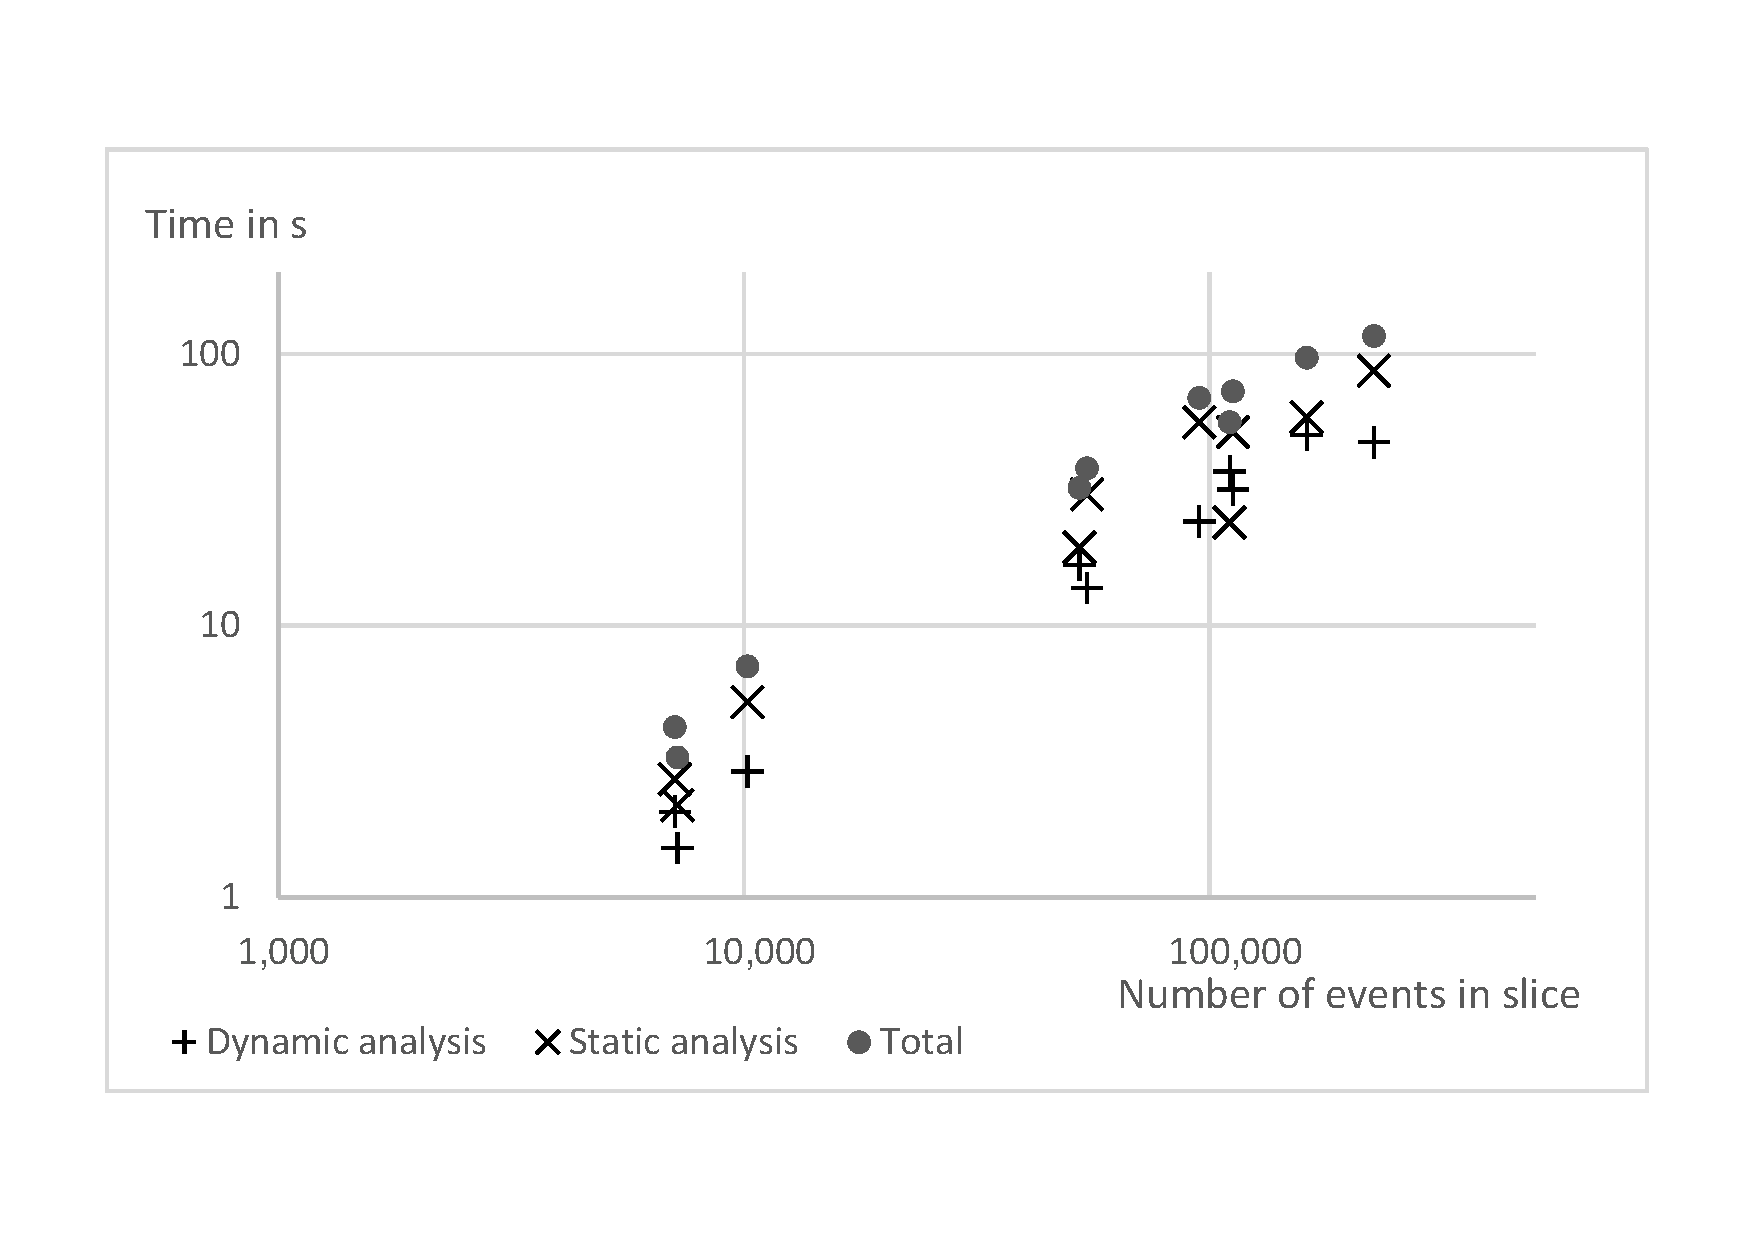
\includegraphics[width=\linewidth, clip, trim={20mm 26mm 20mm 26mm}]{chart-initial.pdf}
	\caption{Time to compute the initial slice}
	\label{fig:chartinitial}
\end{figure}

We previously observed that our approach differs from other slicing implementations insofar as that the run time of the algorithm does not depend on the total length or run time of the sliced program, but only on the size of the resulting slice~\cite{treffer_dynamic_2014}.
Our current measurements confirm that slicing time is linear to the result size.

\Cref{fig:chartinitial} shows the time for computing the initial slice in seconds, depending on size of the resulting slice.
Times are given in total, and divided into static code analysis and the dynamic analysis of the event data.

As can be seen, the static analysis takes slightly more time on average.
It should be noted that the total time is less than the sum of the static and dynamic analysis times, as both can, to some extent, run in parallel,
i.e., while the dynamic slicing algorithm waits for the static dependence graph of one method, the dynamic analysis of other methods can continue.
However, limitations in the Soot framework prevented us from parallelizing the static code analysis.
The chart shows that in our setup the algorithm was able to process approximately 1000 events per second.

\begin{figure}
	\centering
		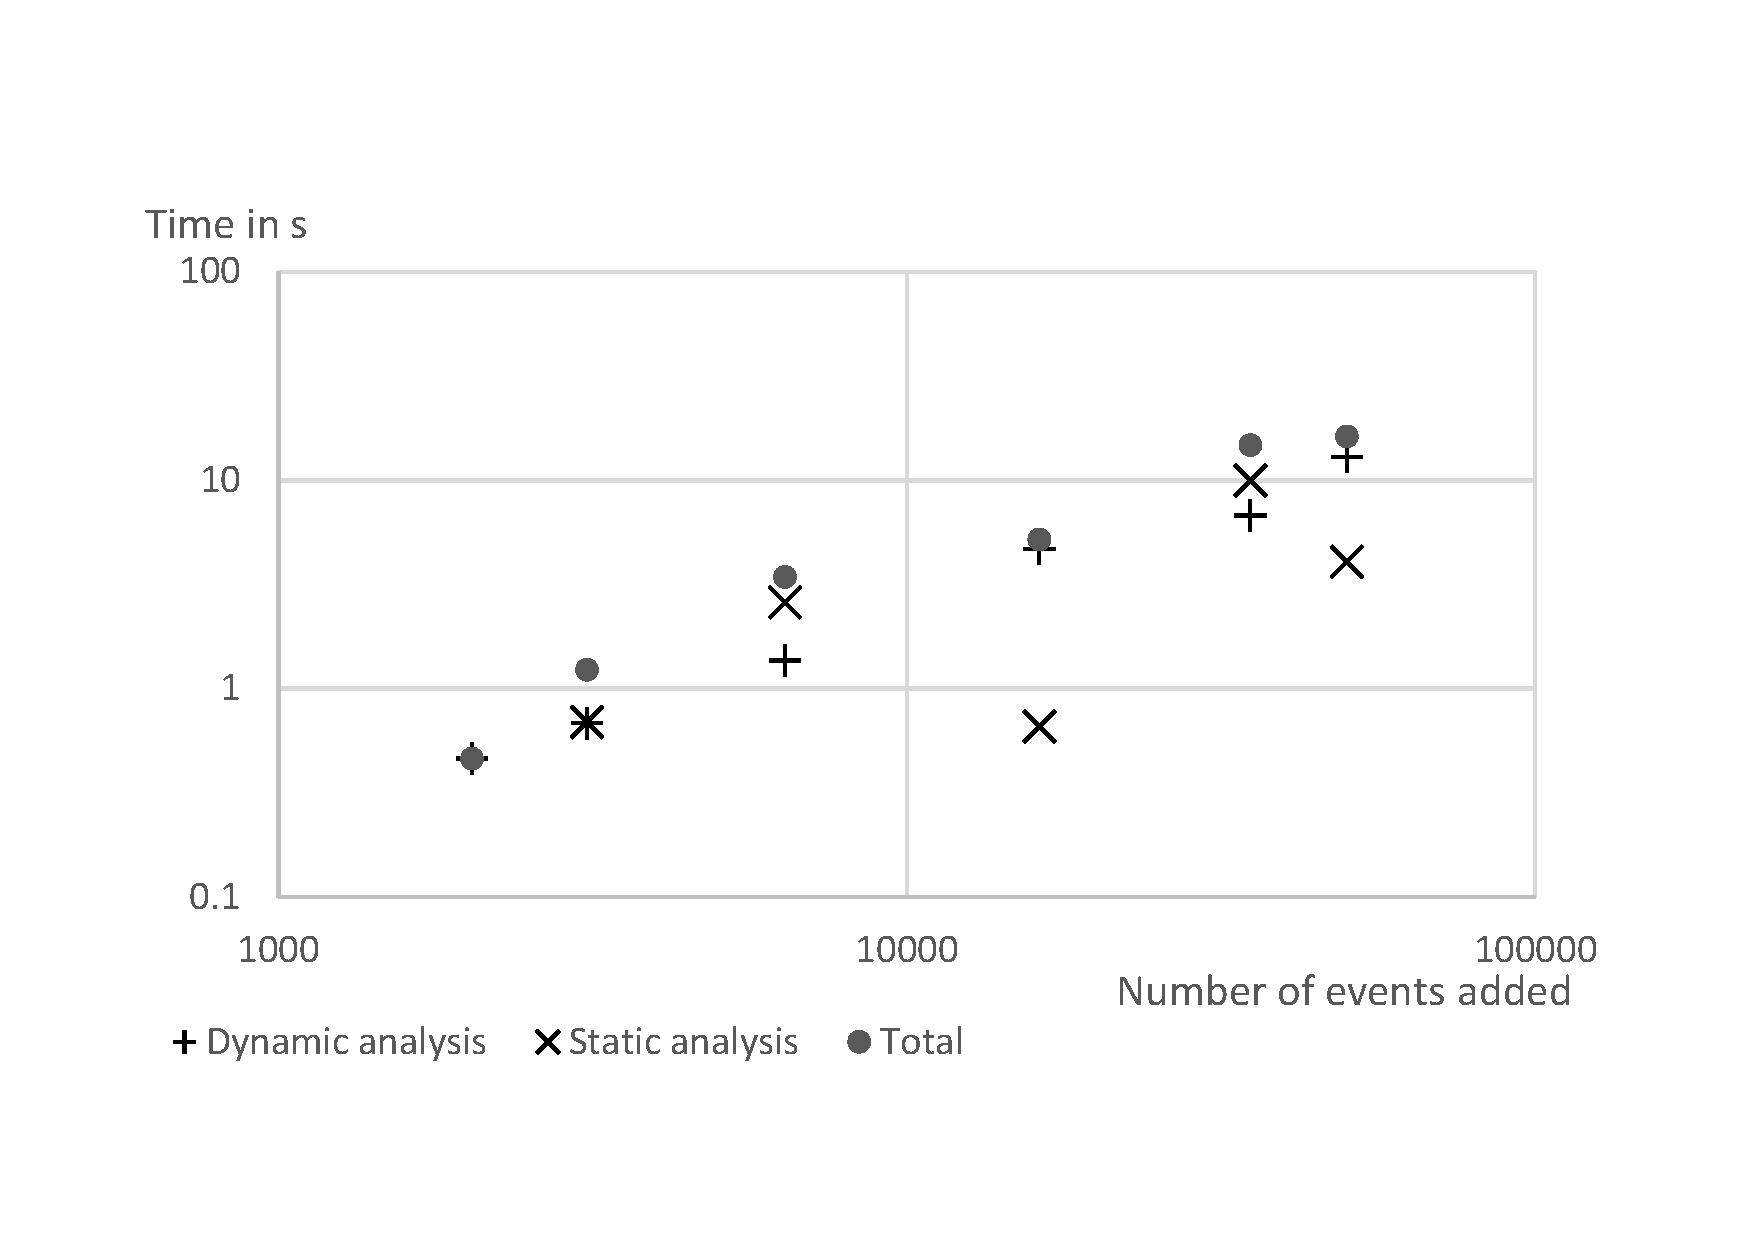
\includegraphics[width=\linewidth, clip, trim={20mm 26mm 20mm 26mm}]{chart-add.pdf}
	\caption{Time to add a slicing criterion.}
	\label{fig:chartadd}
\end{figure}

When adding additional elements to the slice, previously computed dependency graphs can be reused.
As \cref{fig:chartadd} shows, the time for dynamic analysis remains constant per event.
The time for static analysis, on the other hand, shows great variation and depends on how much new code was included by the broadened slicing criteria.
In the worst case, expanding the slice takes as long as creating a new slice for only that criterion.

\begin{figure}
	\centering
		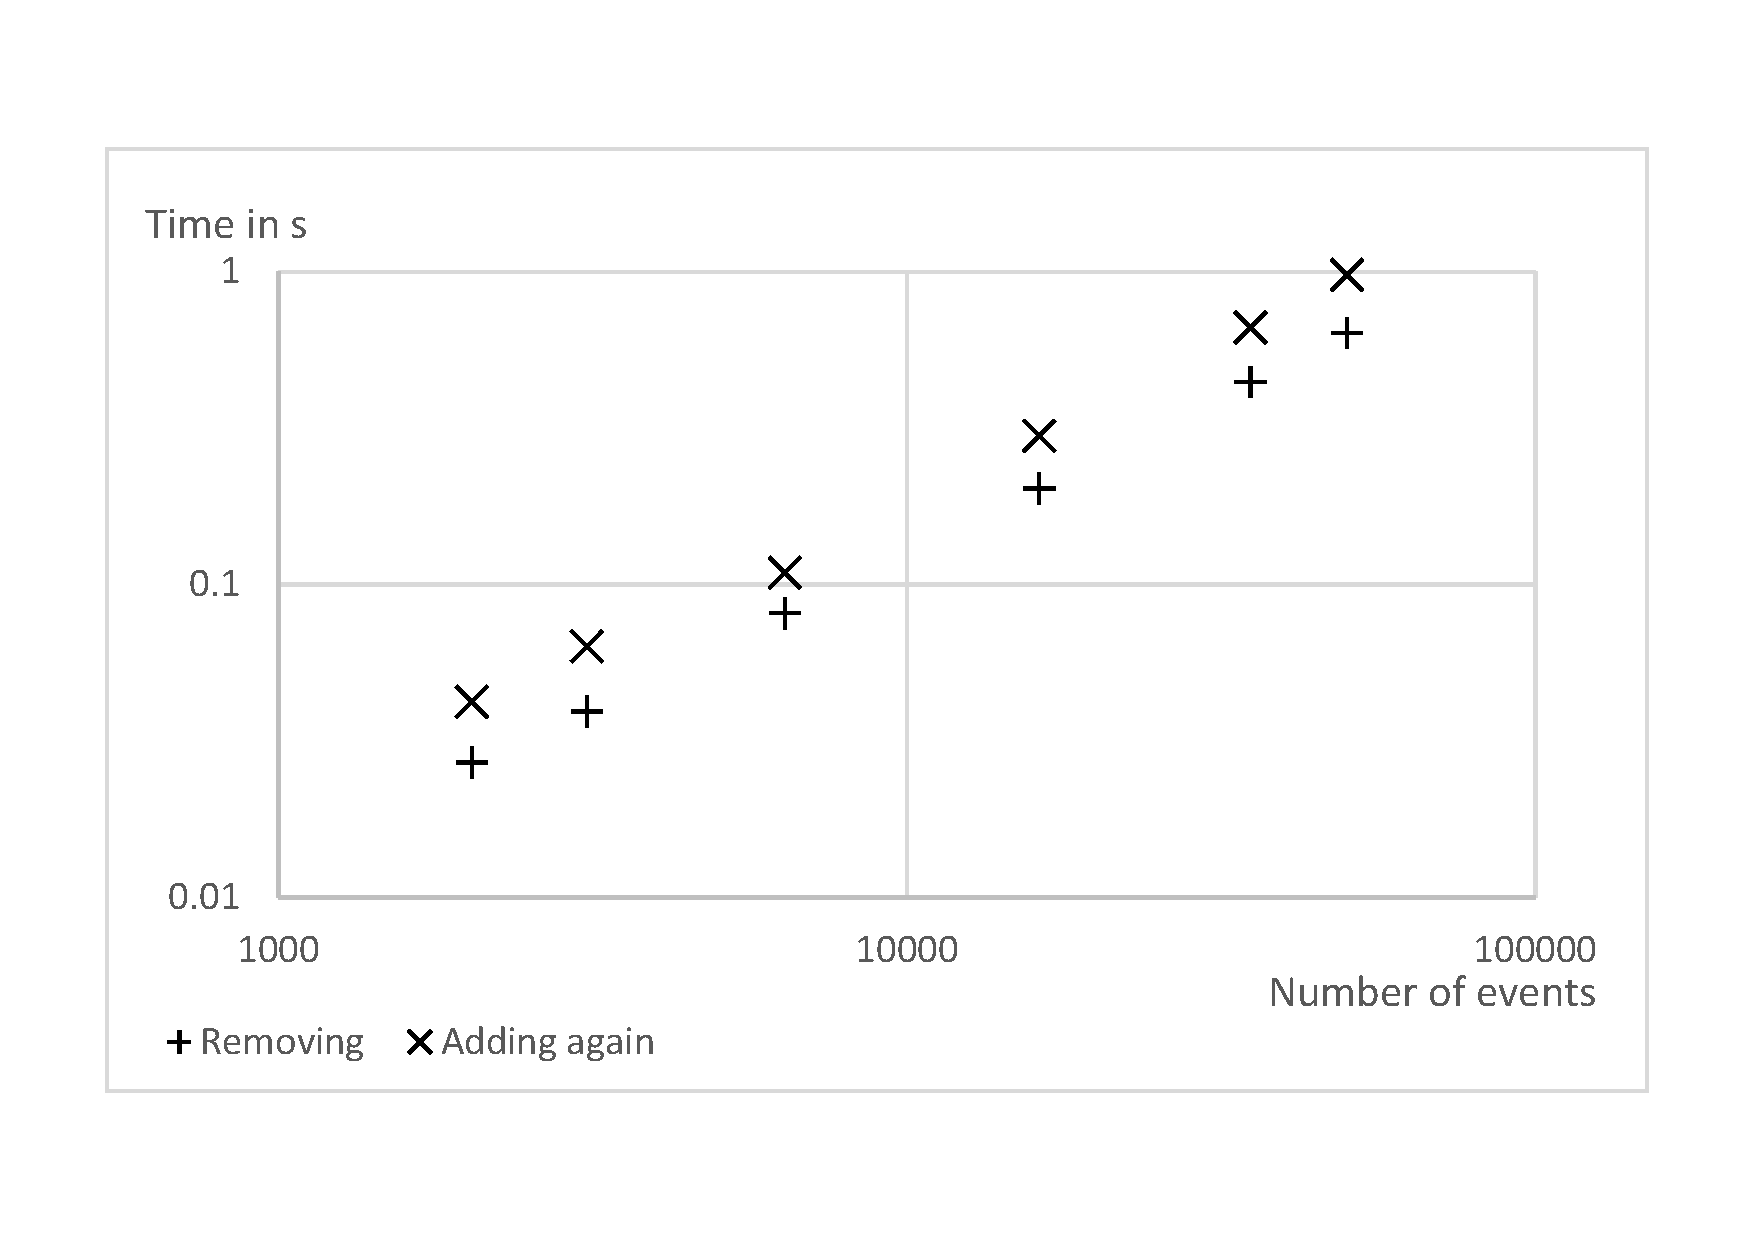
\includegraphics[width=\linewidth, clip, trim={20mm 26mm 20mm 26mm}]{chart-rem.pdf}
	\caption{Time to remove events from the slice}
	\label{fig:chartrem}
\end{figure}

\Cref{fig:chartrem} shows that removing events from the slice by narrowing the slicing criteria is significantly faster, as no complex analysis has to be performed.
Likewise, adding those events again by reverting the slicing criteria change is fast, as previously computed dependency graphs can be reused.

\medskip

From the results in \cref{fig:chartinitial}, it seems as if the slicing algorithm is too slow to be of practical use to a developer.
A single second of execution can produce several hundreds of thousands of events and it is generally not feasible to wait multiple minutes for the slicing to complete.
However, due to parallelization and the design of the algorithm, developers experience a delay of only a few seconds.

As described above, the debugging user interface is updated with an intermediate slicing result twice per second.
The slicing algorithm works its way backwards, beginning at the slicing criteria.
Then, previous events are processed not ordered by their absolute position in the execution, but by their distance in the dependency graph.
As a result, both events from the near past and long-running overarching method invocations are processed first.

This allows developers to begin debugging the slice almost immediately. 
From this point on, they can work unimpeded as long as they don't step backwards faster than the slicer can slice.
If, in the worst case, the slicer is working on many different parts of the program concurrently, then a programmer looking at only one code location might notice a reduced slicing speed.
Additional research is needed to investigate how this phenomenon might manifest in practice.
In all other cases, processing over 1000 events per second should be fast enough to not slow down manual debugging.

For interactive changes of slicing criteria, our experiments have shown that the incremental slicing algorithm is fast enough to not interrupt the developers flow.
In particular, the most common operation -- removing events by narrowing the slicing criteria -- completes in less than a second even for large numbers of events.
From this we conclude that Interactive Dynamic Slicing, based on the Slice Navigator and on iterative slice refinements, is generally feasible.

\subsection{User Study}

To gather empirical data on the usefulness of Interactive Dynamic Slicing, we conducted an experiment where we let developers locate bugs using the regular debugger in the Eclipse IDE, the omniscient debugger from our debugging framework, and the Slice Navigator, and compared their experiences.

\subsubsection{Setup}

We used Defects4J, a database of actual bugs from various open-source projects~\cite{just_defects4j_2014}, to find suitable debugging tasks.
For each bug, Defects4J also provides at least one failing test case and the fix.
We selected bugs from the projects Joda Time, Mockito, and Apache Commons Lang.

Joda Time\footnote{\url{http://www.joda.org/joda-time/}} is a date and time library for Java.
In the version that contained the Defects4J bugs, the project contains 68 thousand lines of code in 157 files.
On top of that, there is a test suite of four thousand tests in 154 files, with 69 thousand lines of test code.
Mockito\footnote{\url{http://site.mockito.org/}} is a Java mocking framework.
The project consists of 14 thousand lines of code in 199 files, and 17 thousand lines of tests in 200 files.
Finally, Apache Commons Lang\footnote{\url{https://commons.apache.org/proper/commons-lang/}} is a library that provides a wide range of commonly needed utility functions that are not implement by the JDK classes.
The library contains 74 files with 48 thousand lines of code, and a test suite of 118 files with 39 thousand lines of code.


%For Mockito and Apache Commons Lang, we selected Defects4J bugs 16 and 53, respectively.

From the Defects4J bug database, we selected Joda Time bugs 10, 19, and 27, Mockito bug 16, and Apache Commons Lang bug 53.
All bugs were selected because they can be fixed with a small change at a single code location and do not require too much knowledge of the technical details of each project.
The three Joda Time bugs affect different parts of the project, so that the order of the bugs will have no impact on the developers' familiarity with the code in our experiment.
Finally, each bug is caused by a different kind of defect.
We expect that the usefulness of each debugging tool varies depending on the nature of the bug.

The first bug is caused by a wrong hard-coded constant value and documented by a test case that fails with an exception.
From an incorrect variable in the \emph{if}-statement that guards the failure-causing \emph{throw}-statement, developers need to follow the infection chain up to the wrong constant.
%The slice for the variable initially contains 324 of the test's 2260 steps.

The second bug is caused by code being missed because of a too restrictive \textit{if}-condition, and is documented by a test case with a failing assertion.
Again, developers must follow the infection chain, but at some point need to realize the state is now entirely correct and conclude that a value should have been changed at some point.
%Slicing on the assertion arguments retains 145 of 465 steps.

The root cause of the third bug is code that gets executed although it should be skipped.
A missing \textit{if}-statement causes a field to be overwritten with am incorrect object reference, which leads to wrong code being called via virtual method calls.
Thus, while following the infection chain developers need to realize that wrong code is executed, conclude that a wrong object is used, and then understand why it was assigned to that field.
Like with the first bug, the test case for bug 3 fails with an exception.
%From the incorrect value in the guardian condition of the throw clause, the slice contains 762 of 3190 steps.

The fourth bug is again a missing \textit{if}-statement that causes a field to be nulled.
However, in this scenario the affected method is executed several times and only in one case nulling the field is an error.
The illegal state is later detected by Mockito's internal validation and causes the test to fail with an exception.

In the fifth bug, wrongly nested \textit{if}-statements cause a method to produce an incorrect return value.
The test checks the value and fails with an assertion error.

We recruited 2 groups of participants for our experiment.
The first group consisted of
twelve full-time software developers with at least 15 years of programming experience, 
four PhD students in computer science with at least 10 years of programming experience,
and eight computer science graduate students with at least 5 years of programming experience who also worked as programmers in a part-time job for at least one year.
The second group consisted of 5 graduate students and 5 full-time software developers with the same levels of experience as in group one, respectively.
Programming experience was self-reported and may include working on software projects in university courses, we asked participants to exclude simple coding exercise in their estimate.
All participants also had experience using the Eclipse IDE for developing Java projects.
%Ages of participants ranged between 25 and 41; two professional developers, one PhD student, and three graduate students were female, all other participants were male.

Every participant was tasked to find the location of a bug by debugging the failing test case with one of the tools.
\Cref{tab:study} shows a summary of all bugs and which tools were tested.
The participants of group one worked on the Joda Time bugs.
No participant had previous experience with Joda Time, although 18 were aware of its existence.
The second group worked on the Mockito and Apache Commons Lang bugs.
Two students had used Mockito before, but not looked into Mockito's internal code.
All participants knew of Mockito's and Apache Commons' existence and general purpose.

For each debugging task, a participant was assigned a bug and a debugging tool.
To prepare for the task, the participant was shown a passing test case similar to the test case they would later have to debug.
We explained the purpose of the test, started the debugging tool to be used,
and let the participant debug the test case, while we explained both the application code and the tool.
When the participant had no more questions, we presented the failing test case and explained the semantics of the failure.
Then we asked the participant to locate the bug using the respective tool and started the timer.
During the debugging session, we provided tool support when needed.
If a bug could not be located within 20 minutes, we aborted the task to advance the experiment.

In the end, in group one every participant had used each tool and every bug was examined with each tool eight times; in group two, because of its smaller size, only the omniscient debugger and the Slice Navigator were used.
With the Slice Navigator, we specifically asked the participants not to use the other features of the omniscient debugger and reminded them during the task if necessary.
This decision was made to prevent participants from ignoring the Slice Navigator and using only the tools they were more familiar with.

% row: 14pt
%\newcommand{\strutA}{\rule[-28pt]{0pt}{28pt}}
% 10 19 27, 16 53
%\begin{table}%
	%\begin{tabulary}{\textwidth}{ccJ>{\raggedleft}p{1.5cm}>{\raggedright}p{1.5cm}}
%%	Bug Nr. & Defects4J ID & \centering Description & \multicolumn{2}{>{\centering}p{3cm}}{Participants\linebreak\small{(Students;Professionals)}} \\ \midrule
	%Bug Nr. & Defects4J ID & \centering Description & \multicolumn{2}{>{\centering}p{2cm}}{Participants} \\ \midrule
	%
	%1 & Time 10 & 
	%Wrong hard-coded constant
	%& DB\linebreak ODB\linebreak SN 
	%& 8 \linebreak 8 \linebreak 8 \cr \midrule
	%
	%2 & f & d & x & 1 \\
	%\end{tabulary}
	%\caption{Relative average time taken for debugging tasks with each tool.}
	%\label{tab:study}
%\end{table}

\renewcommand{\baselinestretch}{1}
\begin{table}%
	\begin{tabulary}{0.97\textwidth}{clC>{\raggedleft}p{1cm}p{0.5cm}}
	Bug Nr. & Defects4J ID & Description & \multicolumn{2}{>{\centering}p{1.5cm}}{Participants} \\ \toprule
	
	\multirow{3}{*}{1}	& \multirow{3}{*}{Time 10} & 
	\multirow{3}{=}{Wrong hard-coded constant} 
	& DB & 8 \\
	&	&	& ODB & 8 \\
	&	&	& SN & 8 \\ \midrule

	\multirow{3}{*}{2}	& \multirow{3}{*}{Time 19} & 
	\multirow{3}{=}{If-condition too restrictive} 
	& DB & 8 \\
	&	&	& ODB & 8 \\
	&	&	& SN & 8 \\ \midrule
	
	\multirow{3}{*}{3}	& \multirow{3}{*}{Time 27} & 
	\multirow{3}{=}{Missing if-statement,\linebreak executed once} 
	& DB & 8 \\
	&	&	& ODB & 8 \\
	&	&	& SN & 8 \\ \midrule
	
	\multirow{2}{*}{4}	& \multirow{2}{*}{Mockito 16} & 
	\multirow{2}{=}{Missing if-statement,\linebreak executed multiple times} 
	& ODB & 5 \\
	&	&	& SN & 5 \\ \midrule
	
	\multirow{2}{*}{5}	& \multirow{2}{*}{Lang 53} & 
	\multirow{2}{=}{Wrongly nested if-statements} 
	& ODB & 5 \\
	&	&	& SN & 5 \\ %\midrule
	
	
	\end{tabulary}
	%\begin{tablenotes}
    %\item[\textdagger] (Students; Professionals)
    %\end{tablenotes}
	\caption{Summary of the tests in our study and number of participants debugging each test with the Eclipse debugger (DB), an omniscient debugger (ODB), and the Slice Navigator (SN).}
	\label{tab:study}
\end{table}
\renewcommand{\baselinestretch}{1.5}

\subsubsection{Comparison of Tool Usage}

\begin{figure}
	\centering %clip, trim={20mm 104mm 20mm 114mm}
		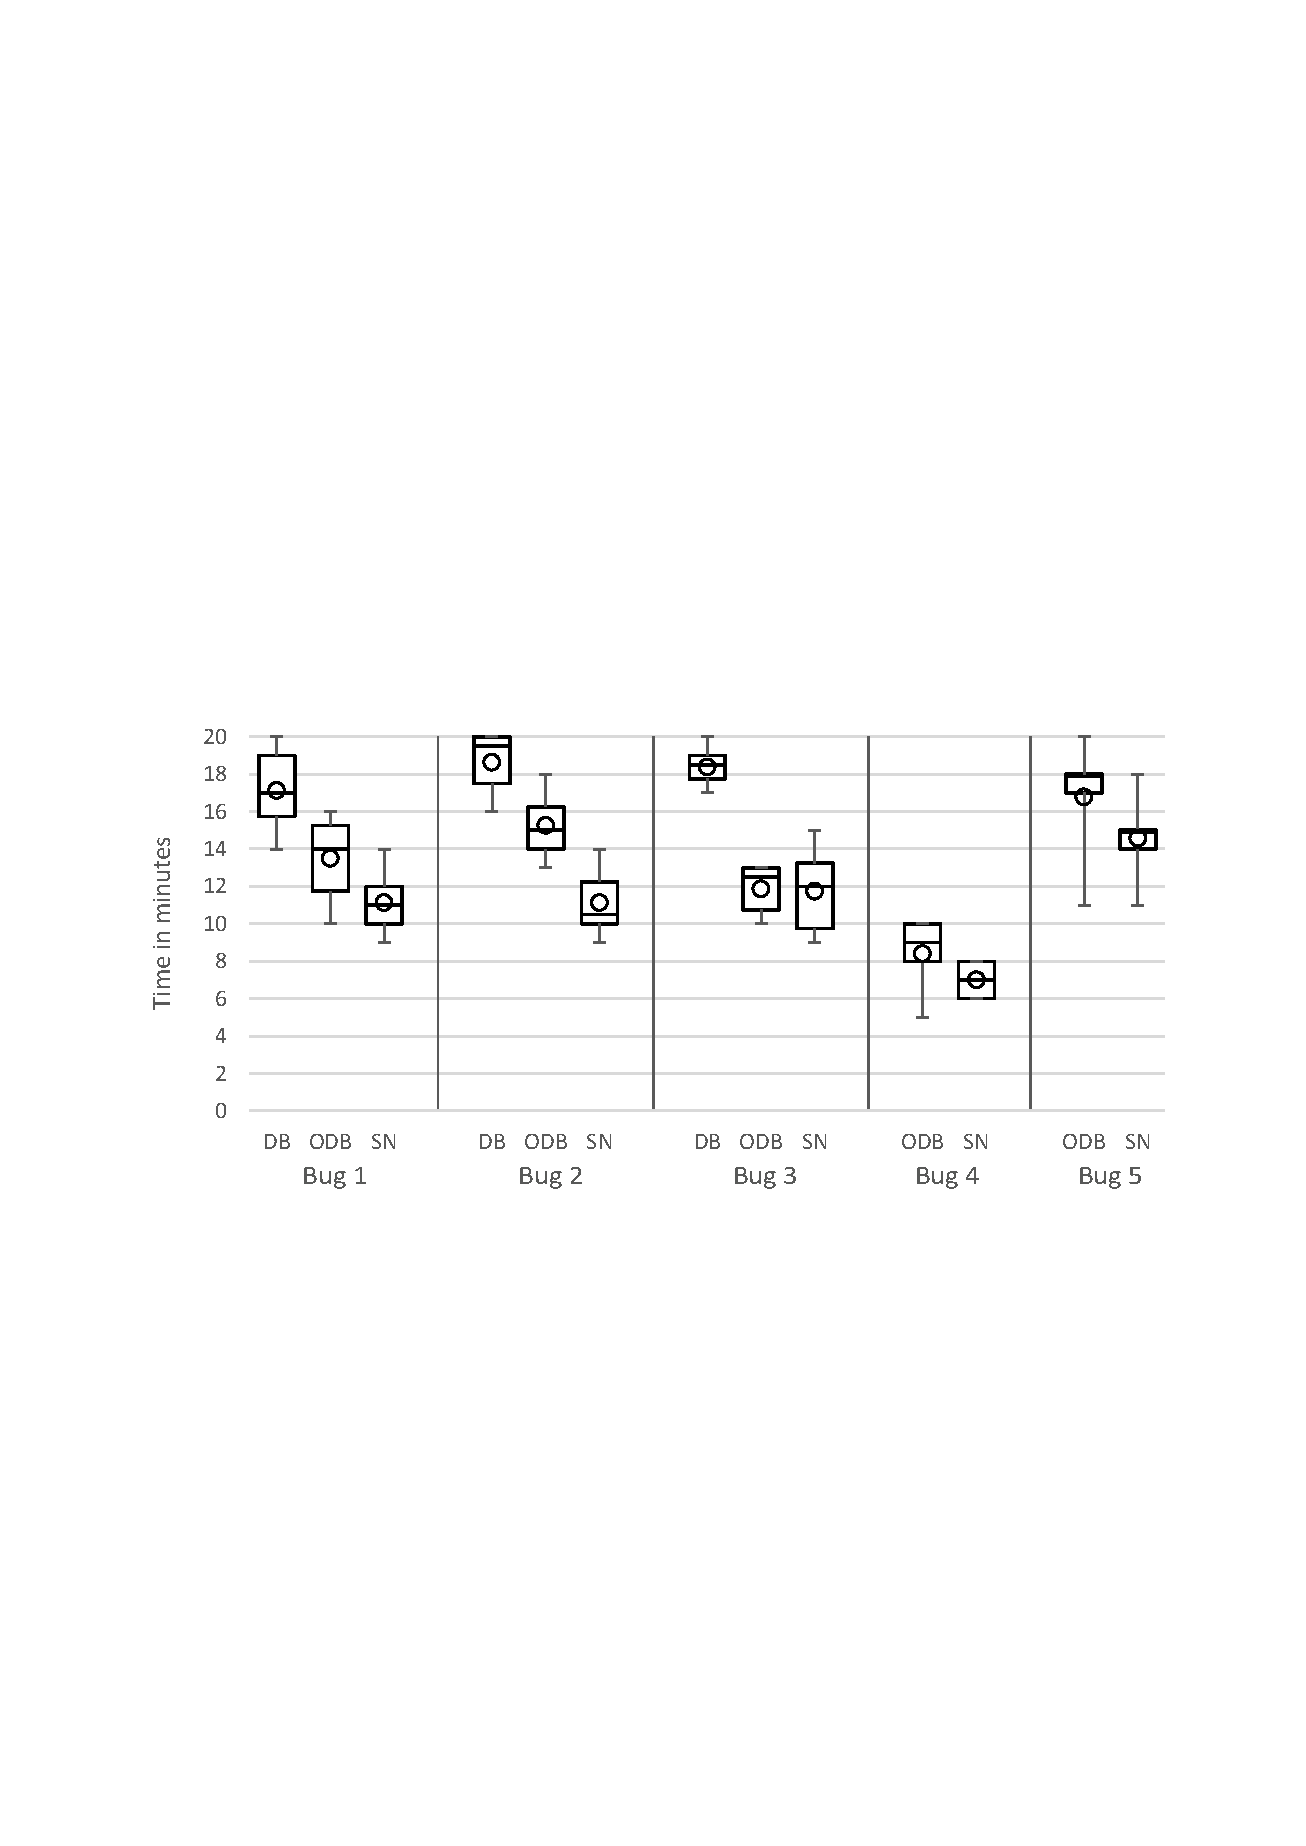
\includegraphics[width=\linewidth]{chart-times3.pdf}
	\caption{Time to solve each debugging task with the regular Eclipse Debugger (DB), the omniscient debugger (ODB), and the Slice Navigator (SN)}
	\label{fig:charttimes}
\end{figure}

\Cref{fig:charttimes} shows the time taken for each debugging task in a box plot chart.
Compared to the regular debugger, the Slice Navigator significantly improved the debugging time for each bug.
Relative to the omniscient debugger, developers using the Slice Navigator were faster with all but one bugs and performed similarly on bug 3.
Furthermore, we observed changes in developer behavior when using different tools.

With the Eclipse debugger, eight participants made heavy use of the "inspect" feature, which evaluates any expression from the source without further executing the program.
In particular, when contemplating whether to step into or over a method invocation, these participants used "inspect" to preview the invocation result.
The participants who used "inspect" had to restart the debugger on average 3.3($\pm0.8$) times, while the other participants restarted on average 8.4($\pm2.3$) times, and noticed they should have stepped into a method immediately after stepping over it 2.6($\pm0.9$) times per task.

Furthermore, 10 participants stopped using the debugger entirely for more than a minute and spent an average of 4.5($\pm1.9$) minutes with pure code reading and mentally simulating the program.
Such behavior was observed with neither of the other two tools.

The omniscient debugger was particularly effective for the third bug, where all but one participants found that a valid field value was overwritten by inspecting the object history.
This allowed them to form a good theory about the nature of the bug very early.
However, the method containing the bug is invoked at two different points in time and each time also calls itself recursively.
The bug occurs only in one of the four executions.
With the omniscient debugger, it took developers a while to notice and distinguish the different invocations as they jumped through time.
Whenever participants expressed confusion related to their current position in the execution time line,
for instance questioning whether an expected operation was already performed or wondering if the debugger jumped to a different invocation of a method, we noted this as being \emph{lost in time}.
Overall, with the omniscient debugger developers felt lost in time 5.4($\pm1.2$) times per debugging session.

Finally, while all developers used the omniscient debugger to step back and forth repeatedly to understand the side effects of a piece of code, 30 of the 34 developers spend most of their time following the infection chain backwards, while four developers mostly debugged forwards in time, like they would with a regular debugger.

With the Slice Navigator, all developers followed the infection chain backwards.
Compared to using only the omniscient debugger, developers were able to reach the end of the infection chain faster, felt lost in time similarly often (on average 5.3($\pm1.9$) times), but took slightly longer to recover from being lost as they had spent less time understanding the code.
However, this draw-back was mitigated by improvements in other areas.
Excluding bug 4, which covered only a small amount of code, developers spent an average of 4.8($\pm1.5$) minutes per task with the regular debugger and 3.4($\pm1.6$) minutes per task with the omniscient debugger, reading code entirely unrelated to the bug.
With the Slice Navigator, this time went down to 1($\pm0.6$) minute per task, leading to better total times.

\subsubsection{Developer Experiences}

After the experiments, we asked the participants how they experienced working with the different tools.

With the omniscient debugger, all participants reported that they found it very helpful to be able to go back and forth in time and felt that they could use it more effectively with more experience, as being used to regular debuggers limited their way of thinking.
Thirty participants said they were at times overwhelmed with the amount of available options and would probably use more of the more advanced features with more experience.
Furthermore, 27 participants expected they would end up lost in time less often with code that they were more familiar with.

For the Slice Navigator, we received similar feedback about moving freely through time.
Furthermore, all participants liked how the Slice Navigator helped to identify relevant program state.
26 participants perceived this as an improvement in particular to the omniscient debugger, as it was less overwhelming.

However, 20 participants found the overarching dependencies shown in gray to be unnecessary and distracting and emphasized the usefulness of being able to double-click an entry to improve the focus of the slice.
On the other hand, 6~participants said they generally liked the idea of seeing relevant state and would probably find it more useful with code they were more familiar with.

Every participant wrongly clicked or double-clicked an entry at least once and was then unable to recover quickly from the mistake.
Thus, an undo-button was requested by all participants.

Finally, 11 participants reported that while the information provided by the Slice Navigator was very useful, they found it distracted from the actual code.
They liked that with a regular debugger they would rarely have to look away from the code and wished for the slicing context to be visualized within the IDE's code editor.

\subsubsection{Discussion}

In our study, we evaluated two contributions: 
First, Interactive Dynamic Slicing, a debugging workflow combining back-in-time debugging and slicing, and second, the Slice Navigator, a debugging tool to support this workflow.

Developers that used "inspect" to look ahead in the regular debugger had to restart their debugging session less often.
This indicates a general need for moving more freely in time.
The addition of slicing was welcomed by all participants, which shows that debugging tools should support not only the navigation of code, but also its understanding.

All criticisms and suggestions for improvement we received concerned only the Slice Navigator, but not the general workflow.
Most suggestions, like the undo-button or a toggle to hide overarching dependencies, are easily implemented UI features.
Even though the user interface still has room for improvements, developers perceived the presented information as helpful for their tasks.

We found a significant improvement in the time needed to locate bugs 1, 2, 4, and 5.
For bug 3, we note that the time needed with the Slice Navigator did not get worse relative to the omniscient debugger, even though we barred users from using the object history view that proved to be very effective for locating this bug.
While the Slice Navigator was not helpful for understanding the root cause in this particular case, it still helped developers to reach the end of the infection chain faster.
Developers wasted less time and, more importantly, less of their memory with reading and understanding unrelated code, leading to similar total times.

Developers getting lost in time reveal a problem that needs further investigation. 
We are not aware of any mentioning of this issue in related literature.
However, it does not seem to be specific to our approach, but rather to indicate a direction where back-in-time debugging in general can be improved.
The idea of showing the information from the Slice Navigator directly in the code may also help developers to recover from being lost more quickly.

On average, using the Slice Navigator developers were 37\% ($\pm9\%$) faster than with the Eclipse debugger and 15\% ($\pm13\%$) faster than with the omniscient debugger.
This suggests that Interactive Dynamic Slicing with the Slice Navigator can make debugging more efficient in many cases.

\subsubsection{Threats to Validity}

External validity is mostly threatened by the size of the study. 
The small number of participants makes it difficult to generalize the results.

Likewise, we only considered five bugs from three libraries.
Although they are real bugs, they all could be tracked down to one location.
For more complex bugs, or bugs in different types of applications, such as web applications, the usefulness of each tool can differ.
To improve the variation, we chose bugs with different characteristics, representing different classes of bugs.

Furthermore, all participants were unfamiliar with the code they had to work with.
Although each participant received an introduction to the code to be debugged, many argued they would have used the tools differently with more familiar code.
A follow-up study should observe programmers using the tools in practice, with full access to all debugging tools at the same time.

Threats to internal validity include the composition of our participant group, which was very heterogeneous with respect to programming experience.
To mitigate this problem, we ensured that participants from each subgroup were distributed evenly across the different debugging tasks.
As \cref{tab:groupresult} shows, students were on average slightly slower using the omniscient debugger and Slice Navigator, but the difference is within the standard deviation of results.
Studies found that computer science students behave very similar to professionals when confronted with new concepts and are therefore suitable for user studies~\cite{host_using_2000, salman_are_2015}.
However, experienced participants from industry appear to use more intuition when identifying important code elements, so some limitations apply~\cite{mcmeekin_significance_2009}.

\begin{table}%
	\begin{tabulary}{\textwidth}{LRRR}
		& Eclipse Debugger & Omniscient Debugger & Slice Navigator \\ \toprule
Students & 98\% ($\pm9\%$) & 79\% ($\pm11\%$) & 66\% ($\pm9\%$) \\
Professionals & 102\% ($\pm7\%$) & 72\% ($\pm\enspace{}9\%$) & 60\% ($\pm7\%$) \\
	\end{tabulary}
	\caption{Average time taken for debugging tasks in group one with each tool, normalized by the average time using the Eclipse debugger on each bug.}
	\label{tab:groupresult}
\end{table}

Internal validity is further threatened by developers gaining experience with the code base throughout the experiment.
We accounted for this by choosing all bugs from different parts of the library in group one and entirely different projects in group two, thus achieving the same level of initial knowledge for each task.

\section{Conclusion}
\label{sec:conclusion}

%Many tools and approaches have been developed to help developers to find bugs in code.
%However, in practice few debugging tools are used that have features beyond symbolic debugging.
Many powerful fault localization tools have been researched in the past decades that have not been widely adopted in practice.
Developers don't like to switch tools while they are in the process of locating a bug and are further deterred by a lack of familiarity.
Short-term memory is limited and important insights are quickly forgotten if attention has to be dedicated to managing tools.

We presented Interactive Dynamic Slicing, a new debugging workflow combining back-in-time debugging and dynamic slicing, and the Slice Navigator, a UI component supporting the workflow and improving the general debugging experience.
Slicing data is used to summarize relevant program state and allows to reach points of interest in the execution history more easily than with breakpoints.
Iterative refinement of slicing criteria allows developers to "forget" about parts of the program that are not of interest.
Combined, these features allow developers to narrow down the cause of a fault efficiently by reducing time and memory spend on code unrelated to the bug.
%Furthermore, the features of the Slice Navigator can be learned over time.
%Developers can start by using only the slicing features, later discover the context visualization, and eventually learn to control the debugger and the slicer.

An evaluation has shown that our algorithms perform fast enough to be usable in practice.
The user study suggests that the Slice Navigator is able to identify relevant state and can improve the efficiency of debugging.
%While the study was too narrow to allow for generalized conclusions, 
While some limitations apply, overall the results and the user feedback are very encouraging.

In our study, we received suggestions for UI improvements that will be implemented as future work.
In particular, the problem of developers feeling "lost in time" needs to be analyzed further.
Even if the problem is less pronounced with more experience with code and tools, better visualizations can help developers navigate through time.
Further research also needs to investigate how much additional context is helpful to developers, especially with regard to overarching dependencies that some developers liked, while others did not.

Finally, we mentioned that configurable slicing can benefit from using dependency types that are useful to the user, but did not discuss what such types could be.
Data and control dependencies followed naturally from the underlying algorithms and seem to model a developer's understanding of a program quite well.
With choice dependencies, we believe we have identified an edge case where more fine-grained control is beneficial.
Following up, further research should show what other dependency relations can be used to better tailor slices to developers' needs.

More general, we argue that combining manual and automatic debugging techniques can create approaches that are more than just the sum of its part and will hopefully help to close the gap between debugging research and practice.
Interactive Dynamic Slicing is a first step in this direction of integrating state-of-the-art research into tools developers use on a day-to-day basis.

%Finally, we wish to bring slicing to database applications.
%With the increasing relevance of "big data", better debugging tools are needed for locating bugs in database applications.
%We expect that slicing can reduce not only the amount of code, but also the amount of data that needs to be analyzed to identify bugs in a program.

%Furthermore, an improved semantic model for well defined interfaces (such as collections in the JDK) can be used to improve the quality of slices. 
%For example, if an add-operation causes the internal array of an array list to be resized, all future "get"s will depend on that "add", even though conceptually only one value was touched.
%

%\nocite{*}

\section*{References}
\bibliography{references}

\end{document}
